\documentclass[12pt]{report}
\usepackage{gensymb}
\usepackage{lineno}
\usepackage{titlesec}
\usepackage{geometry}
\usepackage{lipsum}
\usepackage{caption}
\usepackage{subcaption}
\newgeometry{
    top=1in,
    bottom=1in,
    outer=1in,
    inner=1in,
}
\usepackage{setspace} \doublespacing
\titleformat*{\section}{\LARGE\bfseries}
\titleformat*{\subsection}{\Large\bfseries}
\titleformat*{\subsubsection}{\large\bfseries}
\usepackage{hyperref}
\hypersetup{%makes links, references, and table of contents hyperlinks within the text, and colours them blue
    colorlinks,
    citecolor=blue,
    filecolor=black,
    linkcolor=blue,
    urlcolor=black
}
\usepackage{graphicx}
\usepackage[english]{babel} 
\usepackage[
backend=biber,
style=numeric,
sorting=ynt
]{biblatex}
 
\addbibresource{mybibliography.bib}
\begin{document}
\begin{titlepage}
    \begin{center}
        \vspace*{0.5cm}
        
        \large
        \textbf{Highly Sensitive Atomic Magnetometer For nEDM Experiment }
        
        \vspace{0.5cm}
        \large
        
        
        \vspace{1.5cm}
        by\\
        \vspace{0.9cm}
        Moushumi Das
        \vfill
        
% * <moushumi.das.phy@gmail.com> 2018-09-10T15:56:34.828Z:
%
% ^.
       \vspace{1.5cm}
       A thesis submitted to the Faculty of Graduate Studies of\\ The University of Manitoba\\
       in partial fulfillment of the requirements of the degree of\\
        \vspace{1.2cm}
        MASTER OF SCIENCE
        \Large
        \vspace{0.8cm}
        
%        
\includegraphics[width=0.4\textwidth]{figures/university_logo_}\\
        \large
        Department of Physics and Astronomy\\
        University of Manitoba\\
        Winnipeg
  
        
    \end{center}
\end{titlepage}



\begin{abstract}
%% Text of abstract
A non-zero neutron electric dipole moment (nEDM) would indicate time reversal and charge-parity violation (T and CP). Many experiments are currently being conducted or planned to measure the nEDM. At present the experimental upper bound on the nEDM is $3.0 * 10^{-26}$ e-cm. Our collaboration is developing an experiment at TRIUMF to improve the sensitivity to the nEDM by one order of magnitude ($10^{-27}$e-cm). I am proposed to develop a highly sensitive nonlinear magneto-optical rotation (NMOR) based magnetometer which is a crucial tool in the nEDM apparatus, for stability and homogeneity measurements. The NMOR magnetometer is designed to serve in an array of such sensors to form an auxiliary magnetometer system monitoring the stability and uniformity of the magnetic field in nEDM experiment at the TRIUMF. A NMOR magnetometer has been developed and constructed at the University of Winnipeg. In this NMOR system an atomic vapour cell containing natural rubidium with stable isotopes Rb-87 and Rb-85 is used. An NMOR resonance occurs when the optical pumping is synchronous with Larmor precession. This causes an atomic vapor to become dichroic, so that subsequent probe light experiences polarization rotation modulated at the same frequency. Currently I am working on testing the performance of this NMOR magnetometer.

\end{abstract} 
\pagestyle{plain}
\setcounter{page}{1}
\pagenumbering{roman} 
\tableofcontents
\newpage
\listoffigures
\newpage
\Large
\setcounter{page}{1}
\pagenumbering{arabic}
% page 1 % 

% Chapter 1:  Introduction
\chapter{Introduction\label{ch:intro}}

This chapter will provide some information on why the neutron electric
dipole moment (nEDM) is interesting to measure.  Finding a nonzero
nEDM would answer questions regarding the matter-antimatter or baryon
asymmetry of the universe (BAU).  The measuremet principle of nEDM
experiment and the origin of systematic effects causing false EDM's
will be explained.  This will lead to a discussion on the importance
of magnetometry on nEDM experiment.

\section{CP violation and the Standard Model}

Charge conjugation (C), Parity (P) and Time-reversal (T) symmetry are
discrete symmetries in physics.  C-symmetry describes the symmetry of
physical laws under a particle-antiparticle transformation.
P-symmetry describes the inversion of spatial coordinates and
T-symmetry the direction of time.

CPT-symmetry is believed to be a good symmetry of nature because all
relativistic quantum field theories are invariant under successive
application of the three discrete symmetries.  This is known as the
CPT theorem.

Parity symmetry was discovered to be violated in the weak interaction
through observations of spin correlations in beta-decay.  This is due
to neutrinos having a particular handedness.  This problem can be
fixed proposing that CP-symmetry is a good symmetry of nature.
However, CP-symmetry has also been found to be violated in weak decays
of kaons and B-mesons.

The nEDM is an observable that if found to be non-zero, would indicate
a violation of T-symmetry.  Because of the CPT theorem this is
equivalent to CP-violation.  The current best measurement of the nEDM
gives the upper bound $|d_n|<3.0\times
10^{-26}~e\cdot$cm~\cite{PhysRevLett.97.131801,PhysRevD.92.092003}.
We now discuss how this result impacts physics within and beyond the
standard model.

CP violations in the standard model are arising from two separate
sources.  The first source is found in the strong interaction,
described by the $\theta$ term in the quantum chromodynamics (QCD)
Lagrangian.  This CP violating term in the QCD Lagrangian violates
both parity and time symmetry and induces a nEDM of
$|d_n|\sim-(0.9-1.2)\times
10^{−16}\theta~e\cdot$cm~\cite{bib:chuppetal} with $\theta$ being a
dimensionless parameter of the standard model.  A combination of nEDM
and Hg-EDM measurements limit the parameter to be very small
$\theta\lesssim 10^{-10}$.  The reason for the smallness of $\theta$
is currently unknown.  The second source of CP violation in the SM
arises from a complex phase in the Cabibbo-Kobayashi-Maskawa (CKM)
matrix\cite{PhysRevLett.10.531}.  The phase is responsible for CP
violation in K and B meson decays.  the CP violation within the CKM
matrix predicts $|d_n| = 10^{-31} - 10^{-32}~e\cdot$cm, well below the
current best experimental limit stated above.
%This is known as the
%weak CP-problem since it arises through W boson
%exchange~\cite{PhysRevLett.82.904}.

The T-violating nEDM is considered to be one of the most promising probe for
physics beyond the Standard Model.

\section{Baryon asymmetry}

According to the Big Bang theory, matter and antimatter have been
created in equal amounts in the early universe. But the present
universe is overwhelmingly made up of matter rather than
anti-matter.
% The ratio of baryonic matter to photons can be expressed
%as
%\begin{equation}
%  \frac{n_B}{n_\gamma}=10^{-10}
%\end{equation}
%where $n_B$ is the difference between baryons and anti-baryons number
%and $n_\gamma$ is the number of photons in the Cosmic Backgorund.
The amount of baryon asymmetry generated in the standard model is much
smaller than current observations~\cite{bib:morrissey}.

The Sakharov conditions to explain baryon
asymmetry\cite{budker2013optical}\cite{PhysRevLett.10.531}
\begin{itemize}
    \item Baryon number violation.
    \item Violation of C-symmetry and therefore CP.
    \item Interactions away from thermal equilibrium
\end{itemize}
However, these conditions contain sources of C and CP violation which
haven't been observed so far. Since a non-zero EDM violates CP
Sakrov's conditions would be fulfilled by the existence of a neutron
EDM (nEDM).


\section{Neutron electric dipole moment and CP violation }  
Neutron has an intrinsic electric dipole moment (EDM).  ~The neutron
EDM is a measure for the distribution of positive and negative charges
inside the neutron\cite{wiki:yyy}. Intrinsic EDM of neutron
interacting with external magnetic and electric fields can be
described by the following Hamiltonian:
\begin{equation}\label{my_first_eqn}  
  H=-\mu_n.B-d_n.E
\end{equation}
where $\mu_n$ is the magnetic moment of the neutron interacting with the magnetic field B,and $d_n$ is the electric dipole moment of the neutron interacting with the electric field E.
Since the neutron spin is an axial vector and the electric dipole moment vector is a scalar
vector, both vectors behave differently under P- or T-transformations.  The orientation of the electric dipole moment changes under P operation  but leaves the magnetic moment unchanged. On the other hand, T-operation affects the spin vector but leaves the electric dipole moment unchanged.
 Because of the conservation of CPT symmetry, a non-zero electric dipole moment of the neutron would be a violation of parity (P) and time-reversal (T) symmetry.

\section{nEDM measurement principle}
The Ramsey's method of separated oscillatory fields is the well-known measurement technique
to extract the neutron EDM. In the nEDM experiment, spin-polarized ultracold neutrons, oriented along a uniform field $B_0$ stored into a neutron storage chamber. After applying the magnetic field $B_0$ along the z-axis of the storage cell, the ultra-cold neutrons start to precess about magnetic field $B_0$ at their Larmor frequency.  Then a radio frequency pulse at the Larmor frequency of the neutron is applied to flip the spin by $90 \degree$. The applied electric field is in a collinear orientation to B.  For parallel orientation of E and B, the rotational frequency becomes
\begin{equation}\label{my_first_eqn}  
    h{\omega_0}^ {\uparrow\uparrow}=2\mu_n {B}^{\uparrow\uparrow}+ 2 d_nE
\end{equation}
            
and for the antiparallel orientation of E and B, the rotational frequency is given by
\begin{equation}\label{my_first_eqn}  
    h{\omega_0}^ {\uparrow\downarrow}=2\mu_n {B}^{\uparrow\downarrow}- 2 d_nE
\end{equation}

where $\mu_n$ denotes the neutron magnetic moment, and $d_n$ denotes the hypothetical electric dipole moment. When the value of nEDM is zero, the neutron spin orientation will be anti-parallel to the initial spin orientation but the spin orientation will no longer antiparallel for non-zero nEDM. A fully magnetized Fe-foil is used to detect the neutron spin while transmitting the neutron from neutron chamber which is used to get information about spin orientation. The probability of neutron transmission is proportional to the neutron spin projection on the preferred direction of the Fe-foil. A neutron counter is used to detect the transmitted UCNs. A spin flipper is used to flip the remaining UCNs in the storage chamber in the preferred direction and then they are passed through the neutron counter. An incident for the nEDM is determined from the ratio of the counting rates.

\section{Origin of False EDM}
The dominant sources of systematic error for all previous or proposed EDM experiments come from magnetic field instability (uncorrelated with the electric field E), and magnetic field inhomogeneity through the geometric phase effect\cite{PhysRevA.70.032102}.  The effect is easiest to understand by considering transverse fields originating from the gradient of the uniform $B_0$  field in the axial direction ($\partial B_{0z}/{\partial  z}$).  Now in the presence of electric field E, the experienced additional magnetic field by an UCN particle moving at a speed v on it’s own rest frame can be written as,
\begin{equation}
  B_v = \frac{v\times E}{c^2}
  \label{equation:phase effect}
\end{equation}
 Since the particle moves in the EDM cell, these radial fields also rotate. The rotation frequency of radial field is the same frequency as particles move in the EDM cell.  Therefore, the transverse rotating field induce a phase shift on the resonant frequency from the central value.  This phase shift is known as Ramsey-Bloch-Siegert shift which is proportional to the electric-field strength and therefore mimics an EDM signal. 
 To analyze this effect, the field rotations may be represented in terms of a perturbation on the precession phase. The phase is shifted in 2nd order, resulting in a geometric phase effect.  False EDM effects arise from the interplay between the radial component of the applied $B_0$  field and $B_v$ in the 2nd order perturbation.

\section{ Magnetometry Impact on nEDM}
Ensuring magnetic field stability and homogeneity is one of the key factors to measure nEDM precisely. For that purpose, our collaboration is planning to use dual species comagnetometer inside the UCN cell and an array of highly sensitive all optical atomic magnetometer surrounding the cell. Cesium/Rubidium is used in a set of external magnetometers surrounding the storage chamber.
\subsection{Comagnetometer}
To date,~$^{199}Hg$ is the only atomic element that has been used as a co-magnetometer for a neutron EDM experiment\cite{PhysRevLett.97.131801}\cite{PhysRevLett.102.101601}.  polarized mercury atoms precess in the same volume as the neutrons, hence probing approximately the same space and time-averaged magnetic field.  Comgnetometry is an ideal tool to correct for field drifts.  So 1-10 pT drifts in $B_0$  may be corrected using the comagnetometer technique, setting a goal magnetic stability for the B0  field generation system in a typical nEDM experiment\cite{PhysRevLett.97.131801}\cite{afach:in2p3-01062292}. In nEDM experiment, optical pumping is used to polarize the vapor of mercury atoms. Since the comagnetometer operation is synchronous with the nEDM measurement, injecting polarized mercury atoms and  neutron filling into the precession chamber occurs simultaneously. After the application of a $\pi/2$ pulse, the atoms start to precess freely around $B_0$. When a circularly polarized probe beam interact with precessing atoms the modulation of light intensity occurs and after further analysis of  this effect we get information about Larmor frequency of the atoms. A false nEDM signal may arise due to a combination of a magnetic field gradient $\partial B_{z}/{\partial  z}$ and motion in the electric field when species (neutrons and $^{199}Hg$ atoms) are confined in the measurement cells. In order to avoid the false nEDM problem, our proposed comagnetometer will be based on $^{199}Hg$ and $^{129}Xe$. Xe comagnetometer requires mTorr pressure of pure,
highly polarized Xe in the nEDM cell.
\subsection{Internal magnetometer}

In order to avoid any systematic effects, it becomes necessary to carefully investigate the magnetic field in the UCN storage chamber.  Toward this end, all optical atomic magnetometers will be used in the nEDM experiment at TRIUMF.  These magnetometers, like the mercury co-magnetometer, are scalar so they only measure the magnitude of the magnetic field.  The atomic  magnetometers will be placed in an array surrounding the precession chamber. This arrangement can be used to resolve the multipolarity of field perturbances. Superconducting Quantum Interference Device (SQUID) is one type of highly sensitive commercially available  magnetometer. These magnetometers rely on the superconducting property of trapped magnetic flux. Because of this, they must be operated at cryogenic temperatures. SQUID magnetometers are sensitive to the 0.01 nG level \cite{doi:10.1063/1.3491215}, but keeping a device at extremely low temperatures would be impractical for the nEDM experiment. Spin Exchange Relaxation-Free (SERF) magnetometers boast greater sensitivity than SQUID magnetometers with SERF magnetic sensitivity reaching the 10 fG level\cite{doi:10.1063/1.3491215}. Their limited dynamic range is problematic for non-zero measurements. The most similar in sensitivity to NMOR magnetometers are radio frequency (RF) atomic magnetometers, or MX magnetometers~\cite{Groeger2006}. The basic principle and sensitivity of these magnetometer is same as all-optical atomic magnetometer. A drawback is that the alignment of the atoms crucial to atomic magnetometry are achieved using radio frequency magnetic fields, which again perturb the magnetic
environment, however only at high frequency.  All-optical atomic magnetometers provide a viable solution in combining the perks of each of the previous devices. The most important advantage of using such all-optical atomic magnetometers is that only a polarized laser beam is used to interact with the magnetometer instead of using electrical cables which reduces the risk of additional sources of magnetic fields to the UCN storage chamber. Furthermore, Cs based magnetometers are low  maintenance and they don't have to be cooled with liquid He down to 4 K such as SQUID magnetometer.  The sensitivity of Cs magnetometers can even surpass the sensitivity of SQUID. \\
In this Master's thesis, an introduction into the concept of full optical magnetometry will be presented. This will be continued with a status update, the presentation of measurements with our highly sensitive Rb magnetometer at The University of Winnipeg. 




\newpage
\LARGE
% Chapter 2:  Magnetometry Literature Review
\chapter{Atomic Magnetometry\label{ch:magnetometry}}


 In the following chapter, there will be given an introduction into the quantum mechanical
structure and interactions of a Rb atom with special focus on the hyperfine structure and the Zeeman splitting of the energy levels in an external magnetic field. In the second section of this chapter, the principle of atom-light interactions including optical pumping
will be explained. After introducing basic concepts of alkali atom quantum mechanics, the phenomenology of nonlinear magneto-optical rotation (NMOR) will be discussed, which is the basis for the operation of an atomic magnetometer as it will be used for the nEDM setup

A possible outline of this Chapter.
\begin{itemize}
\item Atomic structure of Rb

Alkali-metal atoms have single electron in their outer shell. For this reason they are often used for optical pumping. Alkali-metal atoms have a nuclear spin.
 Because of the nuclear spin the energy level of these alkali atom becomes complicated.
  \begin{itemize}
  \item g.s.and e.s ($L$, $S$)
  
  
  \item fine structure ($J$)
  
  \item hyperfine structure ($F$)
  
  
  \item Selection rules ($\Delta l$, $\Delta J$, $\Delta F$, $\Delta
    M_l$), D1 and D2 lines of Rb
    
  
  \item Doppler broadening and Rb absorption spectrum (of D1 line)
  \end{itemize}
\item Linear and nonlinear magneto-optical rotation (mostly from
  Budker, Orlando, Yaschuk Am J Phys)
  \begin{itemize}
  \item Hypothetical transition and linear magneto-optical rotation
  
 In the presence of an axial magnetic field, when a linearly polarized light passes through an atomic medium the plane of polarization rotates. This kind of effect is known as the Faraday effect. Afterwards an resonant enhancement of the Faraday rotation has been discovered by D. Macaluso and O.M Corbino in 1898 which is known as nonlinear magneto-optical rotation (NMOR) or nonlinear Faraday rotation \cite{budker2013optical}. Consider an example system of $ F=~1$ to $F'=~0$ transition (Fig~\ref{fig:Zeemansplitting}).  Linearly polarized light can decompose into two counter-rotating circularly polarized components $\sigma^\pm$. The transferable angular momentum is +1 for left circular polarization, -1 for right circular polarization. 
 
 In the absence of a magnetic field, the $M=\pm 1$ sublevels are
degenerate and the optical resonance frequencies for  the two circular
polarizations coincide. 
 In the presence of magnetic field the Zeeman sublevels $M=\pm 1$ shift in energy  by an amount $g\mu B/\hbar$ where g is the Lande factor and $\mu$~is the Bohr magneton. This Zeeman splitting therefore leads to a difference between the  resonance frequencies for for $\sigma^+$ and
$\sigma^-$ light. The left circularly polarized light experiences refractive index $n_+$ and the refractive index for right circularly polarized light is $n_-$. In this case, optical rotation arises due to the difference in the refractive index 
\begin{equation}
\label{eq:emc}
\phi = \pi(n_+-n_{-})\frac{l}{\lambda} \\
\end{equation}
where l is the length of the medium traversed and $\lambda$ is the wavelength of light. The difference between $n_+$ and $n_-$ is shown in  Fig.\ref{fig:Faraday} . On resonance, the rotation is related to the Zeeman shift in the $M=\pm 1$ sub levels. For light with spectral
width of the absorption line much smaller than the transition width, and for zero
frequency detuning from the resonance, the optical rotation can be estimated as
\begin{equation}
\phi \approx \frac{(2g\mu B)/ \hbar\tau)}{(1+((2g\mu B)/(\hbar\tau))^2 )}\frac{l}{l_0}
\end{equation}
where $2g\mu/\hbar$ is correlated to Zeeman splitting, $\tau$ is the doppler width of the
absorption line (of order GHz), and $l_0$ is the absorption length in the medium. 
\begin{figure}[h]
\centering
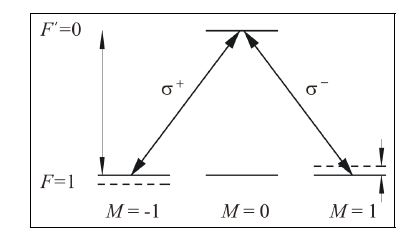
\includegraphics[width=0.75\linewidth]{figures/optical_rotation}
\caption{Illustrative example of F = 1 to $F' = 0$ atomic transition with Zeeman
splitting in the presence of a magnetic field. Image\cite{Budker2002JU2}\label{fig:Zeemansplitting}}
\end{figure}
\begin{figure}[h]
\centering
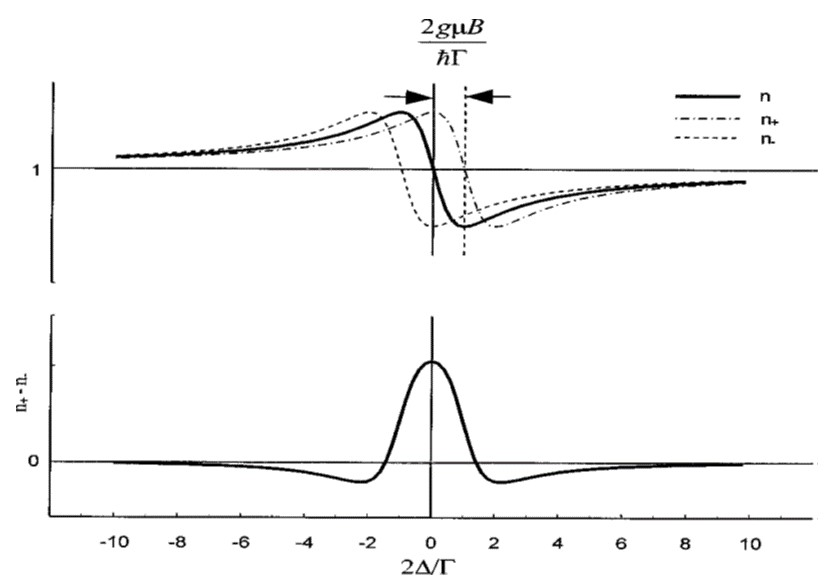
\includegraphics[width=0.65\linewidth]{figures/farday.jpg}
\caption{The dependence of the refractive index on light frequency detuning
D in the absence (n) and in the presence ($n_\pm$) of a magnetic field. Shown is
the case of $2g\mu B=\hbar\tau$ and a Lorentzian model for line broadening. The
lower curve shows the difference in refractive index for the two circular
polarization components. This is the characteristic spectral profile of Macaluso–Corbino opticalrotation. Image\cite{bib:NMOR1998}\label{fig:Faraday}}
\end{figure}
  \item Nonlinear effects in atomic gases: hole-burning and coherent
    population trapping
    

In NMOR, the optical properties of the medium are modified by the laser light, resulting in nonlinear effects such as hole-burning and the creation of a coherent dark state.     
Hole burning is the  nonlinear
effect leading to enhanced Faraday rotation. Spectral holes, or Bennett-structures, are dips in the velocity distribution of a group of atoms produced by pump laser beam. The Faraday rotation produced by atoms with such velocity distribution can be thought of as rotation produced by the Doppler distributed atoms without the hole minus the rotation that would have been produced by the pumped out atoms.

Optical pumping is a process by which light modifies the quantum state of the medium it is transmitting through. Coherent population trapping can be described as the pumping of the atomic system in a particular state, the coherent superposition of the atomic states, which is a nonabsorbing state. The exciting radiation creates an atomic coherence, such that the atom's evolution is prepared exactly out of phase with the incoming radiation and no absorption takes place. In the presence of a magnetic field, the atomic alignment
axis created by the coherent population trapping precesses
around the direction of the field with the Larmor frequency.
  \item Nonlinear magneto-optical rotation; also show result from
    Budker PRL 1998.
  \end{itemize}
\item Magnetometry using NMOR


  \begin{itemize}
    \item Near zero field.
    \item Nonzero field.
      \begin{itemize}
      \item FM NMOR 
      
     
      \item AM NMOR
       

      
      \item Michi's thesis

 
      \end{itemize}
    \item Sensitivity to tilted fields
    
    
    \item Vector magnetometer
    
    
  \end{itemize}
\item Reminder of what we do, leading into next chapter
\end{itemize}


\section{Atomic structure of Rb }
\label{sec:Rb structure} 
The ground state structure of the Rb atom is n = 5, L =0~(s-state) and j = 1/2, i.e, $5^2S_{1/2}$. The lowest excited states (L~=1) are the 5p states. According to quantum theory of angular momentum these 5p states have total electron angular momentum J = L + S where L is the orbital angular momentum and S is the electron spin angular momentum. Fine structure splitting occurs due to spin orbit coupling.  The lowest excited states 5P (L~=1, S=1/2) split into  $5^2P_{1/2}$ and $5^2P_{3/2}$  due to the fine structure splitting. The hyperfine structure is a result of the coupling between J and the total nuclear angular momentum I. The total atomic angular momentum F is then given by F~=~J~+I  and the magnitude of F must lie in the range
$J - I \leq F \leq J + I$. For the ground state of~$^{85}{Rb}$, J = 1/2 and I = 3/2, so F = 1 or F = 2. And  for the excited state $5^2P_{1/2}$ ~  which has nuclear angular momentum I = 3/2 and J = 1/2  the allowed values of F are  1 ~and~ 2. The atomic energy levels are shifted according to the value of F. In quantum mechanics, a set of rules tell us the allowed transition between states which are known as selection rules. The rules are that the total orbital angular momentum change should be $\Delta L= \pm 1$ and the change in magnetic quantum number should be $\Delta M_L= 0,\pm 1$. According to selection rules the transitions from the state L=0 to L=1 are possible. Transmission corresponding to the energy difference between the ~$5^2S_{1/2}$~ and~ $5^2P_{1/2}$ levels of rubidium is termed the D1 line; its wavelength is roughly 795 nm\cite{doe:website}.  The ~$5^2P_{3/2}$~state is separated from the ~$5^2S_{1/2}$~ state by an energy corresponding to 780 nm wavelength, it is called the D2 line. Our Rb atomic magnetometer is based on exciting the D1-line transition by optical pumping.  Linearly polarized laser beam is used to induce transitions of electrons from one energy level to another via optical pumping. In this case, the laser beam is tuned to the transition frequency and of sufficient power to perturb the equilibrium distribution of the ground state energy levels. The gyromagnetic ratio of ${85}^Rb$ is 4.667415 Hz/nT~\cite{bib:rb-gyro-reference}.

\section{Rb magnetometry based on NMOR}

A scalar magnetometer requires coherent precession of the spin ensemble, so a resonant excitation must be applied in order to force some large fraction of the atoms to precess together with a common phase. Otherwise the phase of individual atoms is random, and the total transverse spin of the ensemble averages to zero . The sensitivity of NMOR based atomic magnetometer depends on the lifetime of the polarization state. So in this case, it is important to use ground-state polarization since ground-state polarization has a longer lifetime than the excited states. The working principle of a Rb magnetometer can be described as three step process
\begin{itemize}
\item
Resonant light polarizes Rb atoms via optical pumping. Magnetic
moments of the atoms are oriented with respect to the axis of
alignment
\end{itemize}
\begin{itemize}
\item Aligned magnetic dipole moments experience a torque and precess around the axis of the field at the Larmor frequency and medium becomes birefringent
\end{itemize}
\begin{itemize}
\item A linearly polarized probe beam propagating parallel to the
pump beam is passed through the alkali vapor, the plane of polarization of the probe beam
rotates by an angle proportional to the spin component along that direction, and we detect
this rotation in order to observe the spin behavior. optical polarization rotation of a probe beam is used to measure magnetic field
\end{itemize}
\begin{figure}[h]
\centering
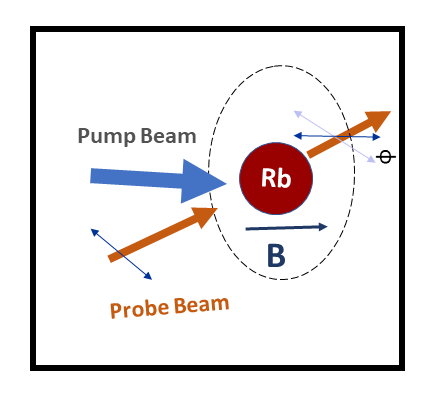
\includegraphics[width=0.55\linewidth]{figures/optical_pumping}
\caption{The schematic diagram of the optical magnetometry technique.
  A linearly polarized pump beam is sent through the vapor cell
  containing natural Rubidium placed in a homogeneous magnetic field
  B.  The polarization rotation of a linearly polarized probe beam is
  used to measure magnetic field,\label{Rb magnetometry}}
\end{figure}

\section{Magnetometry using NMOR}

nonlinear magneto-optical rotation (NMOR), is a promising technique for a new generation of ultrasensitive atomic magnetometers. For magnetic fields directed along the light propagation direction, resonances in NMOR appear when linearly polarized light is frequency or amplitude modulated at twice the Larmor frequency. Because the frequency of these resonances depends on the magnitude but not the direction of the field, they are useful for scalar magnetometry.

 The FM NMOR technique is useful for increasing the dynamic range of NMOR-based magnetometers.  It is possible to achieve the  sensitivity of the device in the range of  $10^{−11} $ G/pHz (comparable or superior, e.g., to the most sensitive superconducting quantum interference (SQUID) sensors)\cite{bib:FMNMOR}.

 Studies have been reported by  Pustelny et al. \cite{bib:AMNMOR,bib:amNMOR} on all-optical magnetometric technique based on nonlinear magneto-optical rotation with amplitude-modulated light. To extent the magnetometer sensitivity to magnetic fields where Larmor
precession is much faster than the ground state relaxation rate, it is
necessary to synchronize the optical pumping rate with Larmor
precession which can be achieved by modulating the light
\cite{doi:10.1063/1.3225917} In AM NMOR, the atoms need to be pumped repeatedly. When this modulation frequency is the same as the harmonic
frequency of the atoms we observe NMOR signal. The method enables sensitive magnetic-field measurements in a broad dynamic range. The sensitivity of  $4.3\times10^{-9}$ G/$\sqrt{\text{Hz}}$ at 10 mG and the magnetic field tracking in a range of 40 mG has been achieved. 

An all-optical magnetometer is also capable of measuring the direction of a magnetic field along with field magnitude \cite{bib:vectormagnetometer}.  This study has been conducted using nonlinear magneto-optical rotation in cesium vapor.  Vector capability is added by effective modulation of the field along orthogonal axes and subsequent demodulation of the magnetic-resonance frequency.  The sensor exhibits a demonstrated rms noise floor of ∼$65fT/ \sqrt {Hz}$ in measurement of the field magnitude and $ 0.5 mrad/\sqrt {Hz}$ in the field direction.  Applications for this all-optical vector magnetometer would include magnetically sensitive fundamental physics experiments, such as the search for a permanent electric dipole moment of the neutron. 

Pustelny et al. \cite{PhysRevA.74.063420}  showed that when the magnetic field is along the light propagation direction, the main resonance occurs at $\Omega_m = 2\Omega_L$. This resonance appear because of the symmetry of the optically pumped state. It is found that when magnetic field direction is tilted in the plane perpendicular to the light polarization axis, resonance is observed at  $\Omega_m = 2\Omega_L$~with its amplitude depending on the tilt angle. In this case, the amplitude of resonance signal decreases with increasing tilt angle . However, If we tilt the magnetic field direction towards the light polarization axis a new resonance appears at $\Omega_L$ along with the main resonance at $2\Omega_L$ if linearly polarized light is used. In this case the resonance signal contain two frequency component Fig \ref{fig:transverse} . The amplitude of the new resonance signal at $\Omega_L$  increases as the angle between B and the light propagation direction increases while main resonance amplitude at $2\Omega_L$  decrease with increasing tilt angle. However,when the tilt angle is larger than some certain angle the resonance amplitude measured at $\Omega_L$ also start to decrease and reaches zero when the magnetic field is directed along the y axis.   It could be possible to evaluate the magnitude of the magnetic field from the ratio of the resonance amplitudes at $\Omega_L$ and $2\Omega_L$. The ratio of the resonance amplitudes at $\Omega_L$ and $2\Omega_L$ can be used to
evaluate the magnitude of the B-field at the measuring point.

 To achieve further sensitivity another way of receiving a signal from the magnetometer
has been studied \cite{mythesis}. In this study an all optical magnetometer has been operated in Free Induction Decay (FID) mode where the Cs atoms have to be excited
once and afterwards the decaying processes (damped oscillation) of the coherence state is
observed (similar to NMR). The sensitivity depends on the T2 time, which is the decay time
of the macroscopic polarization moment.
n self-oscillation mode\cite{PhysRevA.62.043403}, the output signal
of photodiode is fed back to AOM for amplitude modulation. In this
case the output signal of polarimeter is modified to act as a square
wave which drives the AOM directly. After setting the phase and gain
of the feedback system properly, the system start to oscillates
spontaneously at the Larmor frequency. In order to measure the
oscillation frequency a frequency counter can be used in this mode. An
online tracking of the oscillating signal is also possible.

A customized circuit board, consisting of an analog voltage amplifier,
a Schmitt trigger, and two metastable circuits, is used to process
ptical rotation.  {\bf No, it isn't.}

Advantages: Being a quite fast process and having a high bandwidth are
the main features of this self-oscillation scan. In order to get rapid
update of the magnetic field the magnetometer can be operated in this
mode.

%Disadvantages: Since feedback loop self-oscillate in the case of
%constructive interference, it will work only for the signal having a
%phase shift of integer multiple of $2\pi$. This additional phase shift
%might be resulting into slightly off-centered resonance. As a result,
%self-oscillation mode is more susceptible to systematic errors in
%field measurement.


% Chapter 3
\chapter{Overview of Rb magnetometer and apparatus}

\begin{itemize}
\item Purpose: Describe your experiment, focusing on the overall
  function, and providing some description of the individual
  components and their function.
\item Outline:
  \begin{itemize}
  \item Overview of experimental apparatus.  I think this is done by
    describing Figs.~\ref{fig:zerofield} and \ref{fig:pumpprobe}.
  \item Group Fig.~\ref{fig:pumpprobe} into major components and
    describe each one.  For example:
    \begin{itemize}
      \item ECDL and DAVLL
      \item Pump beam and AOM
      \item Probe beam and balanced polarimeter
      \item Cell
      \item Magnetic field system
        \begin{itemize}
        \item Shield arrangement
        \item Degaussing system
        \item Internal coil\underline{s}
        \end{itemize}
      \item DAQ
    \end{itemize}
  \item General operation is discussed in the next chapter.
  \end{itemize}
\end{itemize}

The purpose of this Chapter is to describe the experimental apparatus
used at UW.  I start with an explanation of the overall experiment.  I
then discuss each of the major components of the apparatus in more
detail.


% basic setup and its components,
%the dichroic atomic vapor laser lock (DAVLL), which is used for laser
%wavelength locking to the Cs absorption line will be
%discussed. Followed by an elucidation of the data acquisition (DAQ),

In Chapter~\ref{ch:characterization}, I will cover the initial
characterization of a few different modes of operation of the
magnetometer.  (As discussed in Chapter~\ref{ch:magnetometer}, there
are several different ways in which the magnetometer can be operated
dependent with different advantages and disadvantages to each.)

In Chapter~\ref{ch:results}, I discussed the advances made in the
understanding of the magnetometer performance, mostly in relation to
the development of the Free-Induction-Decay mode of operation.

%this section will be completed with the comparison of different
%possible operation modes of an atomic magnetometer and an introduction
%into the concepts of magnetometer uncertainties and the noise level of
%a measurement

\section{Overview}

\begin{figure}%[h]
\centering
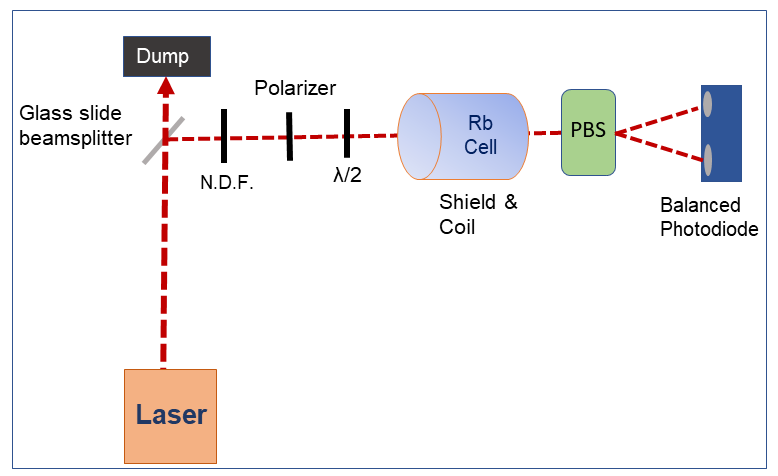
\includegraphics[width=\textwidth]{figures/experimental_setup_zero_field}
\caption{Schematic diagram of experimental setup for zero field NMOR
  measurement.\label{fig:zerofield}.}
\end{figure}

Fig.~\ref{fig:zerofield} depicts the zero-field apparatus.

Fig.~3.2 depicts the layout of the system used in the Physics
Department of The University of Winnipeg for studying the non-linear
magneto-optical effects with the amplitude modulated light. In this
work, a paraffin-coated vapor cell (about 5 cm long) containing
natural rubidium with stable isotopes $Rb^{87}$ and $Rb^{85}$, is used
as the magneto-optical sample. To get maximum sensitivity and to
reduce ambient fields the cell is placed within a magnetic shield made
of four-layer of $\mu$ metal. This magnetic shield is capable to
provide passive attenuation of dc magnetic fields by a factor of
$10^6$. A semiconductor diode laser is the light source. The laser
wavelength ($\lambda=795$ nm) is precisely controlled by an external
locking system and its radiation is amplitude modulated by an
acousto-optical modulator.  The light beam is splited into pump and
probe beam using a beamsplliter. The typical light power of the pump
beam is 40 $\mu$W and the typical light power of the probe beam is 20
$\mu$w. Upon passing through the Acousto Optic Modulator (AOM) and
linear polarizer linearly polarized light beam interact with Rb
atoms. The probe beam then passes through our vapour cell which sits
inside the shield. Then the nonlinear Faraday rotation signals are
analyzed by a balanced polarimeter.  A Wollaston prism is used to
split the beam into its perpendicular polarization axes which are then
analyzed individually by our photodiode. Our photodiode contains two
individual diodes and an internal differential amplifier which outputs
the difference in diodes P1 - P2. A lock-in amplifier was used to
detect the polarimetric signal and stored on a computer.
\begin{figure}%[h]
\centering
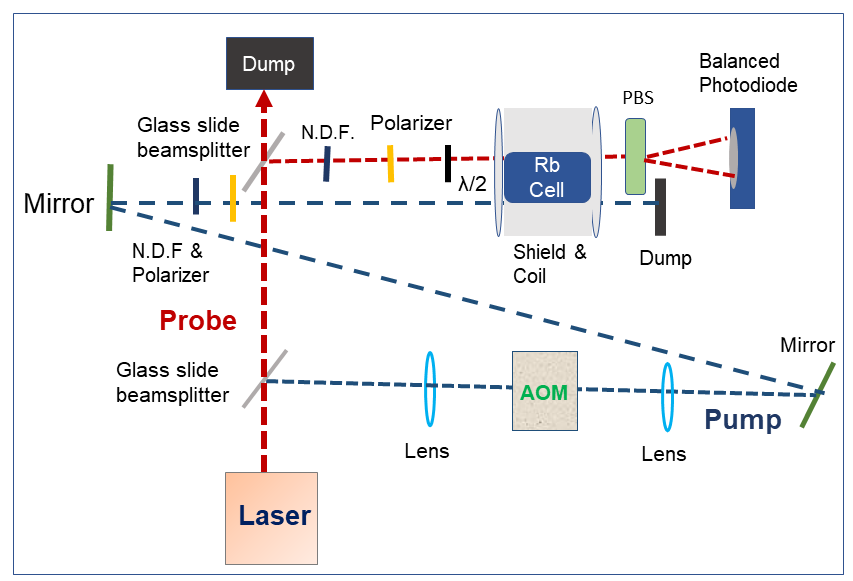
\includegraphics[width=0.95\linewidth]{figures/experimental_setup}
\caption{Schematic diagram of the experimental setup for measuring
  rotation of the polarization plane with amplitude modulated (AM)
  light. AOM stands for acousto optic modulator, $\lambda/2$ - half
  wave plate, N.D.F- neutral density filter, PBS- polarizing beam
  splitter.\label{fig:pumpprobe}}
\end{figure}
\section{External Cavity Diode Laser(ECDL)}
\bigskip
In our NMOR based optical magnetometry setup, laser light was provided by an external cavity diode laser. These kind of diodes are semiconductor diodes and thus vibration and shock resistant. They are also wavelength tunable. ’Besides that, external cavity diodes emit single mode laser light with a very narrow-band linewidth. A critical aspect of an ECDL is temperature control of the cavity, since the laser frequency depends on the cavity length and hence on the thermal expansion coefficient of the cavity material. Micrometer screws enable manual coarse tuning, while precise scans without mode hops are performed by a piezo actuator. This kind of grating stabilized diode lasers is especially advantageous for spectroscopy with the alkalines. Our Toptica DL-100 outputs a tunable wavelength near 795 nm with an output power $<100$ mW. The laser spot size is elliptical, and approximately 3 mm x 5 mm = $15 mm^2$.The laser was typically tuned to the D1 (F = 3,2 2) absorption minimum and then adjusted to maximize optical rotation. Our NMOR system uses an atomic vapour cell containing natural rubidium with stable isotopes $Rb_{87}$ and $Rb_{85}$ both being present.

\section{Dichroic Atomic Vapor Laser Lock (DAVLL)}
\medskip
In order to control the laser frequency to a fraction of the linewidth of the atomic transition of the Rb D1-line, a frequency error signal is generated by taking usage of the Zeeman effect combined with circular dichroism of an atomic vapor which is exposed to a magnetic field \cite{doi:10.1063/1.3568824}. The generated error signal passes through zero crossings as the laser frequency coincident with the lock frequency. A linearly polarized probe beam is incident on a glass cell filled with Rb vapor surrounded by a set of permanent magnets. The wavevector of the light is parallel to the axis of the generated magnetic field by permanent magnets. After the interaction of the laser beam with the Rb cell, the beam passes through a quarter-wave plate before impinging on a polarizing beam splitter (PBS) or a Wollaston prism. The linearly polarized beam incident can be split into two orthogonal circularly polarized beams. A set of photodiodes are used to detect the intensity of the right and left circularly polarized beams. Both of the photodiodes are attached to a polarimeter board which is used to measure the difference in signals and amplifies it. One oscilloscope is used for monitoring each photodiode as well as the difference output. The signal is then fed into a PID controller which finally controls the laser diode current corresponding to a certain laser frequency.
\begin{figure}[h]
\centering
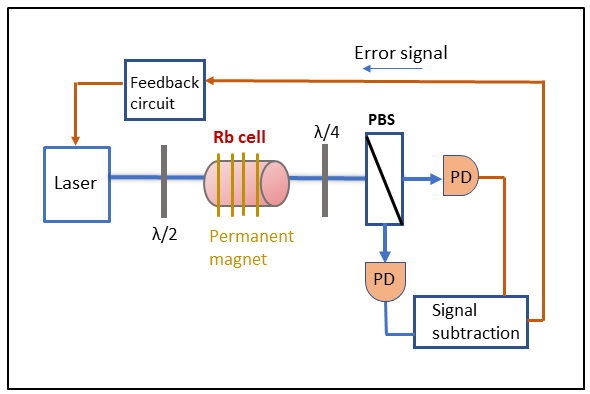
\includegraphics[width=0.8\linewidth]{figures/DAVLL}
\caption{Schematic diagram of experimental setup for characterizing the DAVLL . PBS- polarizing beam splitter, PD- photodiode.}
\end{figure}

\section{Acousto-optic Modulator (AOM)}

The acousto-optic modulator offers a method of modulating the
amplitude of the light.

\begin{itemize}
\item What's it for, in this experiment?
\begin{itemize}
\item Used for pump beam.
\item Pump beam sets the state of the atoms.
\item Linearly polarized light, so modulated at $2\omega_L$.
\item Enforces precession of axis of alignment in order to form a
  coherent state.
\item After a while the AOM is switched off for probing the state.
\end{itemize}
\item How does it work?
\begin{itemize}
\item I think you have most of this below.
\end{itemize}
\item What are the parameters used in our experiment?  How do we
  really use it?
\begin{itemize}
\item Our particular AOM model \# and parameters of that model and
  driver.
\item How we drive it with a function generator.
\item Focusing, alignment, max intensity of the 1st order Bragg.
\item operation frequency in 0.2 uT, 1.0 uT field.  Bandwidth of the
  AOM itself.  Delay time after function generator signal.
\end{itemize}
\end{itemize}





This method works for both phase and amplitude modulation of light.
In order to measure the magnetic fields in the far of the zero-field
regime, an amplitude modulated pump beam needs to apply to the
magnetometer.  This amplitude modulation is done by a square wave
modulation with a duty cycle of 1-10\%.  This additional modulation is
accomplished with an acousto optic modulator (AOM).
\begin{figure}[h]
\centering
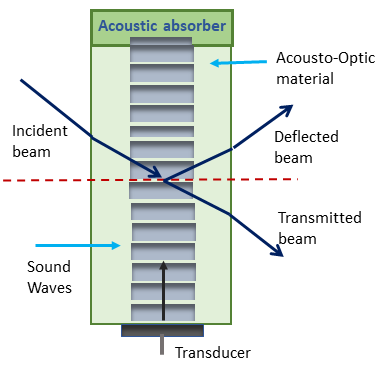
\includegraphics[width=0.7\linewidth]{figures/AOM}
\caption{Acousto-optic modulator}
\end{figure}
In principle, it contains an optically transparent medium (e.g glass, quartz) which has a piezoelectric transducer attached at the end that propagates acoustic waves within the medium. An RF signal needs to apply to the transducer to generate the acoustic wave. The compressions and refractions of the sound waves result in periodic variations of the refractive index of the medium which then form a diffraction grating. Any incident laser beam will be diffracted by this grating generally provides a number of diffracted beams. The strength of the sound wave is directly related to the intensity of the defracted light. Depending on the interaction length L, laser wavelength $\lambda$ in the medium and the sound wavelength it is possible to operate AOM in two different modes: 
\begin{itemize}
\item  In the Raman-Nath regime ($L<\Lambda^2/\lambda$) many orders of diffraction are possible. The maximum intensity of the first-order diffracted light (relative to the incident light) is only about 35\%. Due to this relatively low efficiency, this type of AOM is used as a loss modulator fo r intracavity applications which require that light is removed from the zero-order diffraction or that a beam is straight propagating through the device e.g. Q-switching.


\end{itemize}
\begin{itemize}
\item In the Bragg regime($L > \Lambda^2/\lambda$) the light beam enters the medium at one particular Bragg angle 
\begin{equation}
\theta_B=\frac{\lambda}{2\Lambda}
\end{equation}                                 
and only one diffraction order produce. This observed diffraction pattern generally consists of two diffraction maxima; these are the zeroth and the first orders. In this case the possible maximum intensity of the first order diffracted light is 100\%. Due to this relatively high efficiency, this first order can be used for amplitude modulation. For our atomic magnetometry setup we operated the AOM in the Bragg regime.

For this prototype setup, an AOM driver is used with an RF center frequency of 80 MHz. The AOM uses crystal tellurium dioxide ($TeO_2$) for the optical interaction medium and Lithium Niobate as the piezoelectric transducer. The amplitude modulating pulses are driven with TTL signals, generated by an Agilent 33522A function generator. This AOM has a bandwidth of 80 MHz\\


\end{itemize} 
\section{Magnetic Shielding}
In precision magnetometry, magnetic shielding is required to achieve well characterized, stable magnetic field conditions independent of the earth’s magnetic fields and environmental perturbations. Shielding ratio T is a parameter to evaluate the efficiency of a shield which can be expressed as
\begin{equation}
 T = \frac{B_{in} }{B_0} 
\end{equation}

where $B_0$ is the homogeneous magnetic field in free space, and $B_{in}$ is the field induced in the presence of shield due to  $B_0$. Using multi-layer shielding is an efficient way to enhance shielding efficiency\cite{doe:website2} . The effectiveness of a multilayer shield with thin shells having wide gaps between them is same as the much heavier and more expensive thick, single layer shield.
The optimization of the air gaps between the shells is important to minimize the total size of a multilayer shield. When a coil is placed inside the innermost layer of passive shield the shield turns into a return yoke. As a result, the magnitude of field $B_0$ increase. A four layer $\mu$-metal magnetic shielding with nearly spherical geometry is used for this highly sensitive Rb magnetometer. $\mu$-metal is a very high permeability nickel based alloy, which is used for shielding low-frequency magnetic field. When the shape is close to a sphere we will get zero magnetic field inside independent of the outside field. The inner radius of the innermost shield is 18.44 cm, equal to its half-length. The radii and half-lengths of the progressively larger outer shields increase geometrically by a factor of 1.27. Each cylinder has two endcaps which possess a 7.5 cm diameter central hole\cite{Andalib:2016ahj}. A stove-pipe of length 5.5 cm is placed on each hole was designed to minimize leakage of external fields into the progressively shielded inner volumes. The magnetic shielding factors of each of the four cylindrical shells, and of various combinations of them, were measured and found to be consistent with $\mu_r \sim 20, 000$\cite{Martin:2014foa}
\begin{figure}[h]
\centering
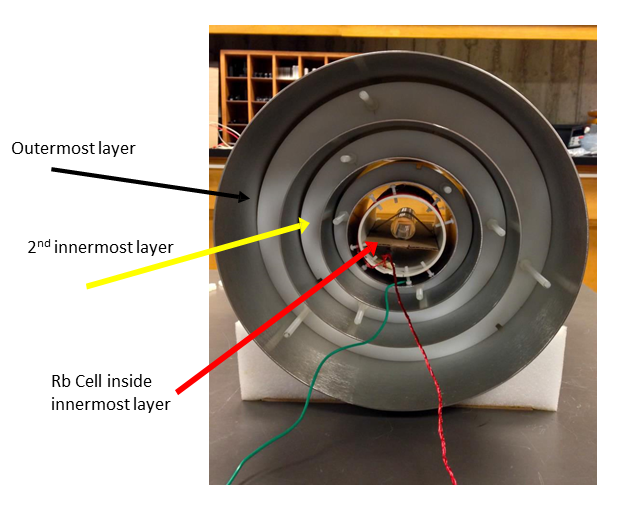
\includegraphics[width=1.0\linewidth]{figures/magnetic_shielding}
 \caption{Four layer $\mu$ -metal magnetic shielding.The diameter of
each endcap is larger by 0.1 cm to fit over its corresponding cylinder. The hole diameter and stovepipe length for each endcap are the same. High
density polyethylene spacers and nylon thread rods/nuts are used to hold the shields and end caps together.}
\end{figure}
\newpage
\section{Rb Cell}
When glass cell is used to store alkali atoms, the atomic mean free paths increase and alkali spins depolarize immediately after making non-elastic collision with the glass walls.
Prolonging the atomic alignment is crucial to achieving ultra-narrow NMOR
resonance widths. So it is necessary to prevent these non-elastic collisions for achieving the longer lifetimes of atomic ground state coherences \cite{PhysRevA.72.023401}\cite{Balabas:10}  \cite{doi:10.1063/1.3236649}. Two methods are currently in use to extent the atomic coherence lifetime. One of them is to add buffer gas to the cell containing alkali sample and the other method is to coat the inner walls of the cell with anti-relaxation materials. The advantage of using buffer gas is that it reduces the resonance width by extending the lifetime of coherence state. A paraffin-coated vapor cell containing  natural rubidium with stable isotopes $Rb_{87}$ and $Rb_{85}$ is used for this work. The reason behind using paraffin as a anti-relaxation coating is that it allow polarized atoms to bounce off the walls of a paraffin-coated cell $\sim 1000$ times before depolarizing\cite{PhysRev.147.41}\cite{PhysRevA.72.023401}. Coated cells have the advantages of providing larger optical rotation
signals, reducing the effect of magnetic field gradients on the spin polarization lifetime,
and lowering the power requirements of the lasers used for pumping and probing. The vapor cell is cylindrical, 5 cm long and 5 cm in diameter with optical
flats on the ends. The cell was provided by D. Budker, having been prepared in
a fashion similar to the cells described in Ref.\cite{PhysRevA.72.023401}. The cell was characterized
using a method similar to Ref. \cite{PhysRevA.72.023401}, by measuring the relaxation of longitudinal
polarization using optical rotation as a probe. The long time component of the
relaxation was thereby found to decay with a time scale of 60 ms.  Longer relaxation time indicates good quality of cell. The temperature of the vapour cell was controlled by the ambient temperature of the surrounding room (∼ 21 $\deg$). Transmitted light was analyzed for optical rotation by a balanced polarimeter system containing a Wollaston prism and a Newport model 2307 balanced photo receiver. The power delivered to the vapour cell was typically 15 $\mu$W, measured periodically using a Newport Model 818-SL power meter inserted into the
beamline. 
\begin{figure}[h]
\centering
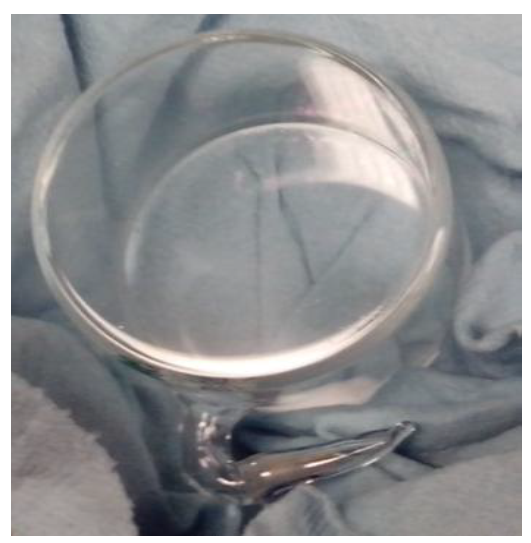
\includegraphics[width=0.5\linewidth]{figures/cell}
\caption{Paraffin coated Rb cell}
\end{figure}
\newpage
\section{Internal coil}
 For the Rb atomic magnetometer an internal coil is used to provide the magnetic field. This coil produces uniform field in the ROI of magnetic shielding, directed along the axis of the cylindrical volume. The coil was wound on a 7.62 cm diameter, 20.32 cm long ABS plastic pipe. Seven turns of 26 AWG magnet wire were wound at 2.54 cm spacing, with 1.27 cm spacing from the magnetic faces of the endcaps of the innermost magnetic shield. The spacings were chosen so that, in the infinite permeability limit, and in the limit where the axial aperture holes in the endcaps are small, the boundary conditions would produce image currents forming an infinitely long solenoid . This is similar to the design strategy used in Ref. [16]. Two saddle coils were wound on the same cylinder in order to control transverse fields internally; these were normally disconnected during precision measurements. The internal coil system was calibrated using a three-axis fluxgate magnetometer at fields of ∼100 nT. This fluxgate was too large to fit through the end caps of the shield, so calibration
had to be performed without end caps. The calibration of the z-coil was verified using the NMOR magnetometer with an AM pump beam, and the known gyromagnetic ratios of Rb-85 and Rb-87. Homogeneity of the residual field and magnetic field generated by the coil system was measured by scanning a fluxgate magnetometer along the axis of the system with and without the coil energized. At a field of 1 $\mu$T, the axial field generated by the coil was uniform within the ROI to the $1\%$  level.
\section{Lock in Amplifier}
SR830 DSP Lock in Amplifier is a elementary part in the DAQ system of Rb magnetometry. It can measure very  small voltages. The most attractive feature of a lock in amplifier is that it is able to suppress all noise contributions which differ from the reference frequency. A reference signal is applied to the lock-in amplifier which is usually done by an external oscillator which passes a discriminator. In this magnetometry setup sync output of a function generator is used as external reference signal for force oscillation scan. The external reference signal is phase locked to an internal reference frequency, provided internal oscillator of the lock-in.Since a lock-in amplifier has two phase sensitive detectors we obtain two output signals. During the process of phase sensitive detection (PSD), the reference signal is first multiplied with the real input signal  and in a second stage, the real input signal is multiplied by
the lock-in reference signal with a phase shift of $90\degree$. Then a lowpass filter is used to filter both signals .The first one is referred to as X output and the 2nd output signal is referred to as Y output. X output is knows as in phase component and the Y output is called out of phase component.
\section{Degaussing system(need to edit)}
Our four layer $\mu$ metal magnetic shield is designed to minimize the magnetic field at the cell, but
magnetic hysteresis limits the magnetic field in any region to be exactly zero. Degaussing (demagnetizing) process is used to reduce the background magnetic field inside the shield. Although Rb cell is securely placed inside the four layer mu-metal shielding it is necessary to demagnetize the shield before every measurement session  to eliminate accidentally created local magnetizations.
Demagnetizing is achieved by winding a special coil around inner most layer of shielding  in toroidal configuration
and supplying the coil with oscillating current. An Agilent 3522A function generator  provides a ramped sinusoidal that controls a current supply driving the degaussing coil \cite{Martin:2014foa}. The wires going to the degaussing loop should be twisted together to avoid picking up or causing noise. Switch is opened to electrically disconnect the degaussing coil.
 
\begin{figure}[h]
\centering
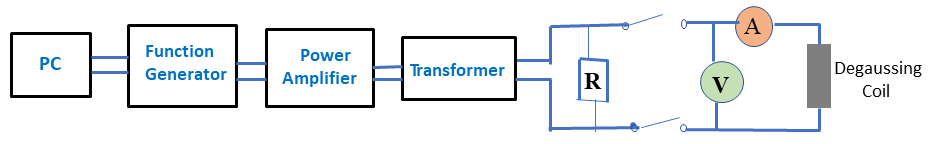
\includegraphics[width=1.0\linewidth]{figures/degaussing_system}
\caption{Schematic diagram of degaussing System}
\end{figure}

\section{Signal Processing(need to edit)}
For small optical rotation, the rotation angle $\theta$ is given by 
\begin{equation}
\theta=\frac{p_1-p_2}{2(p_1+p_2)}
\end{equation}
       
where $P_1$ and $P_2$ represent signals of the two photodiodes in the polarimeter. The differential value is acquired with a lock-in amplifier (LIA) referenced to the pump beam modulation provided by a function generator. The demodulated signal from the LIA is acquired by a personal computer for analysis. 
\section{Laser tuning and locking}
In order to polarize atoms by optical pumping, it's important to tune the laser properly to expected transition line.
Setting the laser temperature correctly is one of the important parts to achieve good tuning . First we need to turn on the temperature control panel and then it’s easy to adjust laser temperature manually by tuning the knob of temperature control panel. For our tune the laser temperature is set to 20.1 $\degree C$. For good tuning it is also important to know the laser current which corresponds to the emission of laser light with a wavelength matching the absorption line of the Rb atom. This is usually done by a DAVLL scan so it's necessary to make sure the DAVLL optical setup is done correctly. An oscilloscope is used to observe the output of the differential amplifier. Trigger the scope on the trigger output on the sweep control panel.
Laser current can be controlled by adjusting the current control knob until the spectral structure of Rb -85 appears. we need to keep adjusting the current control knob until a maximum symmetry between the upsweep and downsweep portions is achieved. After that by adjusting the knob of sweep control panel we can zoom in the structure and set the trigger to steep of the absorption minima. 


Digilock 110 feedback controlyzer is used for laser locking. The DigiLock 110 is an up-to-date digital hardware allows to implement the scan generator, PID controllers and optional frequency modulation techniques all into one plug in module. It offers graphical user interface running on a PC makes the procedure of laser locking enormously easy. Different important features are also available in this module for analyzing and optimizing the control system.
 
The output of the laser feedback controlyser panel is connected to the computer where Digilock software was already installed. The output signal of the differential photodiode is fed into the controlyser panel main input. After connecting the DigiLock 110 we can turn on scan and navigate to the autolock screen at the bottom. Then the the portion of the spectrum that we tuned earlier will appear. Then we need to select the crosshairs tool which allow us to drag the crosshairs on the part of the spectrum that we want to tune to. Finally for successful laser locking we need to click and select "PID lock to slope".
\begin{table}[h]
\centering
\begin{tabular}{|l | l|}
\hline

\textbf{ Position}    & \textbf{Laser Power} \\
\hline

AOM &   $4mW$  \\

Pump beam   &    $60\mu W$  \\

Probe beam   &    $22\mu W$  \\
After Cell  &      $18\mu W$   \\

\hline
\end{tabular}
\caption{Adjusted laser power at several positions in the experiment}
\end{table}


% Chapter 4
\chapter{Magnetometer Operation\label{ch:characterization}}

In this Chapter I describe the different ways in which the
magnetometer was operated.  Some of these modes of operation were
applied to furhter experiments, which are reported in
Chapter~\ref{ch:results}.  Some of the modes were simply used to
perform a basic characterization of the magnetometer and to compare
with the results of other groups which were discussed in the
Literature Review in Chapter~\ref{ch:magnetometry}.

The main purpose of this Chapter is to give an overview of the many
parameters which can affect the performance of the magnetometer.
Chapter~\ref{ch:results} goes into further detail on studies of
specific performance metrics under modification of additional
parameters.

The main operation modes of the magnetometer reported in this Chapter
are:
\begin{itemize}
\item Near-zero-field operation.  In this mode, the magnetic field
  must be swept in order to calibrate the magnetometer.  The dynamic
  range of the magnetometer in this case is $|B_z|\lesssim 0.2$~nT.
\item Amplitude modulated NMOR, which itself was used in two distinct modes:
\begin{itemize}
\item Continuously pumped (a.k.a.~forced oscillation) mode.  In this
  mode, the amplitude of the pump beam was modulated continuously and
  the optical rotation signal was demodulated resonantly at the same
  frequency.
\item Free-induction decay (FID) mode.  In this mode, the amplitude of
  the pump beam is modulated for a time and then switched off.  The
  oscillation frequency of the optical rotation signal is then
  measured non-resonantly.
\end{itemize}
In these modes, the magnetometer was generally operated at 0.2~$\mu$T
or 1.0~$\mu$T, which is of considerably more relevance to the nEDM
experiment.
\end{itemize}
In Chapter~\ref{ch:results}, most of the measurements will relate to
our studies using FID mode.  The exception is that some degaussing
studies will be done near zero field and hence will use that mode.


\section{NMOR near zero field and degaussing studies}

During this measurement the pump beam was switched off and the probe
beam is used as its own pump (see
Section~\ref{sec:something-in-chapter-3}).

I used the magnetometer in this mode to study the function of the
degaussing system described in
Section~\ref{sec:Degaussing}.

The experiment was carried out as follows:
\begin{enumerate}
\item The laser beam was tuned for maximum optical rotation and
  stabilized using the DAVLL system.  The beam power was $\sim
  20~\mu$W.
\item Optical rotation of the probe beam was monitored throughout the
  experiment via an oscilloscope monitoring the differential
  photodiode signal.
\item The innermost magnetic shield was degaussed with various
  parameters for the sequence.  The operation of the degaussing
  circuit was described in Section~\ref{sec:Degaussing}.  After
  completing the degaussing sequence a switch is opened to
  electrically isolate the degaussing coil.
\item The magnetic field along the $z$-direction (defined in
  Section~\ref{sec:Internal coil}) is swept in order to calibrate the
  differential photodiode signal as a function of applied $B_z$.  In
  this way the initial magnetic field after degaussing may be deduced.
\end{enumerate}
%In this case,  at first degaussing the shields that surround the vapour cell is done in order to cancel background B-field.A function generator is used to drive the degaussing coil. After completing a degaussing sequence switch is opened to electrically disconnect the degaussing coil from experimental setup. Then B-field ramp is started and NMOR signal is observed through a oscilloscope which  connected to balance photodiode output. The magnetic field sweeping is done in a triangle wave. In 
Fig.~\ref{fig:TUNE} displays the sequence of measurement events in
time, along with the differential photodiode signal (in Volts), which
is proportional to optical rotation.  Also shown is a voltage applied
to the $z$-coil with a 10~k$\Omega$ resistor in series which dominates
the resistance of the circuit.  Recall that the coil constant of the
$z$-coil is $\sim 48$~nT/mA (see Section~\ref{sec:Internal coil}).
The sweep range of this trace is therefore
% (0.8~V)/(10000~Ohm)/*48~nT/mA = 3.84 nT ???  It would be good to
% write the correct calibration constant in the part of the thesis
% where this coil is describe (probably somewhere in Chapter 3).
1.9~nT peak to peak.

In the first section of the oscilloscope trace, the impact of the
degaussing procedure inducing noise in the optical rotation signal can
be seen.  The next section involves the ramping down of a variable
resistor, followed by opening the switch to isolate the degaussing
coil.  Then the magnetic field $B_z$ is swept and the characteristic
dispersive Lorentzian shape of NMOR is observed.

\begin{figure}%[h]
\centering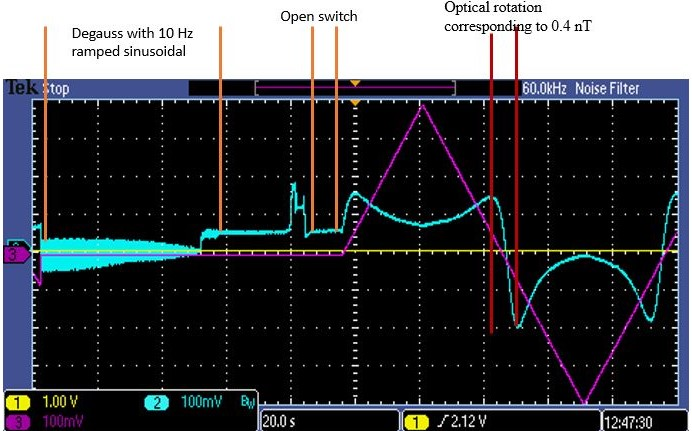
\includegraphics[width=0.7\linewidth]{figures/scope_trace_of_field_sweeping}
\caption{Oscilloscope trace of measurement OR near zero field. The
  purple curve shows the voltage across the 10~k$\Omega$ resistor in
  series with the $z$-coil, from which the magnetic field ramp of
  1.9~nT peak to peak can be deduced.  The blue trace indicates the
  differential photodiode signal which is proportional to the optical
  rotation.  The left side of the traces show the impact of the
  degaussing procedure, while the right side shows the calibration
  procedure.\label{fig:TUNE} }
\end{figure}


In this measurement NMOR signal is used to determine effectiveness of
degaussing procedure. After the degaussing procedure the observed OR
signal is non-zero while the applied field $B_z$ was zero which
indicates the existence of a remnant field.  The effect of degaussing
parameters sensed by the magnetometer is discussed further in
Section~\ref{sec:degaussing}.


% We need to have this table somewhere, but I think it needs to be in
% the section where you talk about degaussing.

%\begin{table}%[h]
%\centering
%\begin{tabular}{|l|l|}
%\hline
%\textbf{SETTING}    & \textbf{VALUE} \\
%\hline
%Function generator &   \\
%\hline
%Frequency &  10 Hz   \\
%Sample rate    &  10000 sample/sec  \\
%Amplitude   &   10 V \\
%Offset  &       0 V  \\
%\hline
%\end{tabular}
%\caption{Setting for degaussing \label{table:degaussing setting}}
%\end{table}

Fig.~\ref{fig:near zero field} shows an example of the calibration of
the differential photodiode signal to the field applied by the
$z$-coil, for data where the degaussing part of the sequence have been
removed.  The field is calibrated to the voltage signal as described
above.  In Fig.~\ref{fig:near zero field}, the data have been fitted
to a dispersive Lorentzian shape given by the function
\begin{equation}
\mathrm{Signal~(V)}=\frac{A(B-B_0)}{somefunctionthatMoushumifillsin}
\end{equation}
where $A$, $B_0$, $a$, and $o$ are fit parameters.  A key measure of
magnetometer performance is the valley-to-peak distance, which in this
case is about $\Delta B=\frac{2}{a}=0.49$~nT.  The other key measure
in this case is the deduced field at zero crossing given by the fit
parameter $B_0=0.019$~nT.  Thus, after degaussing, a remanent field of
19~pT is found.  This is only the on-axis field.  It is possible that
transverse fields can be larger, and these tend to make the width
$\Delta B$ of the zero-field curve larger.

\begin{figure}[h]
\centering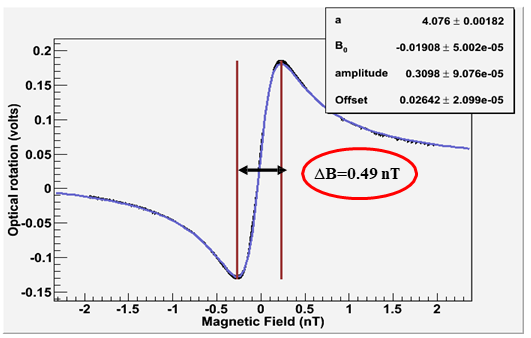
\includegraphics[width=0.7\linewidth]{figures/near_zero_field}
\caption{Optical rotation as a function of magnetic field applied
  along the direction of the laser beam. The signal looks like a pure
  dispersive Lorentzian curve. The measured resonance width is 0.49~nT
  and the measured remanent field is 0.019~nT.\label{fig:near zero
    field}}
\end{figure}

In order to determine the sensitivity, a magnetometer can be operated
in different modes. Most of them found its application during the time
this Master's thesis was prepared. Although main focus of this work
was to study magnetometer performance in Free Induction Decay (FID)
mode.

\section{Amplitude Modulated NMOR:  Forced Oscillation Mode}

In this forced-oscillation measurement scheme the pump beam amplitude
is modulated and the differential photodiode signal is demodulated at
the same frequency $\Omega_m$ using a lock-in amplifier.  The
modulation/demodulation frequency is near twice the Larmor frequency
of the atoms in the magnetic field.

In the first instance, we tried keeping the frequency constant and
sweeping the magnetic field.  We can then determine the resonant field
by fitting the resonance lineshape.  The disadvantage of this method
is that the field must be changed in order to measure it.  {\bf An
  example of this might be shown in Fig.~\ref{fig:AMORmaybeidontknow},
  or it might not be.  Really, it is impossible to tell.}

\begin{figure}[h]
\centering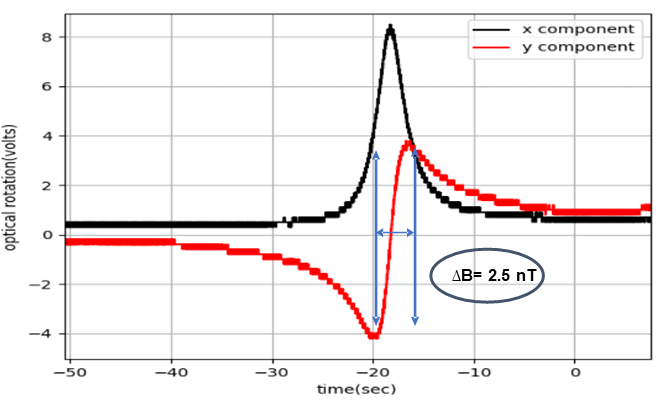
\includegraphics[width=0.7\linewidth]{figures/AM_NMOR}
\caption{\bf The rest of this figure caption might be totally
  false... AMOR resonance signal with a 5 cm cell containing natural
  Rb.  Data was acquired by using a balanced photodiode which
  demodulated through lock-in amplifier as the frequency is swept
  slowly near 9.37~kHz.  The parameters of the sweep are shown in
  Table~\ref{tab:freqsweep} and are discussed further in the text. The
  observed resonance width, when translated from frequency into field,
  is 2.5~nT.\label{fig:AMORmaybeidontknow}}
\end{figure} 

A better way to measure the field without having to change it is to
sweep the modulation/demodulation frequency instead.  The resonant
frequency then gives a determination of the field (when
$\Omega_m=2\Omega_L$)

\begin{figure}[h]
\centering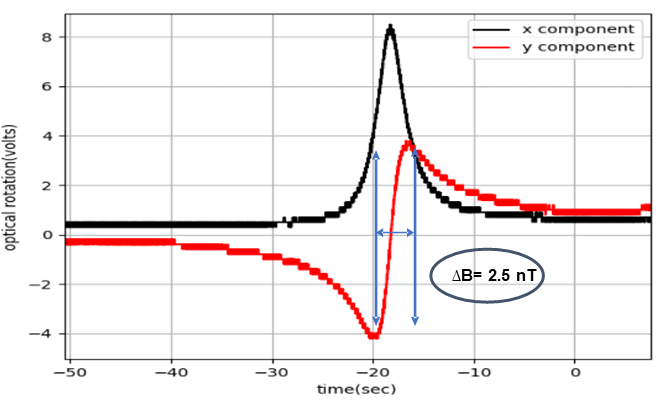
\includegraphics[width=0.7\linewidth]{figures/AM_NMOR}
\caption{\bf I do not know what this figure is, and so here is what
  I'm guessing that it might be: AMOR resonance signal with a 5 cm
  cell containing natural Rb.  Data was acquired by using a balanced
  photodiode which demodulated through lock-in amplifier as the
  frequency is swept slowly near 9.37~kHz.  The parameters of the
  sweep are shown in Table~\ref{tab:freqsweep} and are discussed
  further in the text. The observed resonance width, when translated
  from frequency into field, is 2.5~nT.\label{fig:AMOR}}
\end{figure} 

Fig.~\ref{fig:AMOR} {\bf potentially, maybe, and if it doesn't we
  should find the figure that does show this, since you included the
  table below which relates to the data that may or may not be
  presented in the figure but should be} shows a measurement of the
in-phase and quadrature signals measured while the frequency is swept
very slowly.  The parameters of this mode of operation, particularly
of the slow frequency modulation, are shown in
Table~\ref{tab:freqsweep}.

\begin{table}%[h]
\centering
\begin{tabular}{|l |l|}
\hline

\textbf{ SETTING}    & \textbf{VALUE} \\
\hline
Function generator &   \\
\hline
Frequency & 9.37kHz   \\

Waveform    &  Square  \\

Amplitude   &  $1V_{pp}$  \\
Offset  &       500 mV  \\
Duty cycle       &    $1\%$ \\
Frequency Deviation     &   40 Hz  \\
FM Frequency     &   100 mHz  \\
modulation waveform      &    Triangle \\
Amplitude modulation & On \\
\hline
Lock-in amplifier &     \\
\hline
Lock in frequency     & 9.37 KHz \\
Time constant     &  $300\mu s$ \\
Sensitivity      &  100mV  \\
\hline
\end{tabular}
\caption{Setting for AM NMOR at $1\mu$T field {\bf which may or may
    not correspond to any other data showed in any other figure of
    these thesis.  All other parameters of the measurement are
    apparently unknown.}.\label{tab:freqsweep}}
\end{table}

Fig.~\ref{fig:AMOR} shows the characteristic dispersive and absorptive
shapes in the in-phase and quadrature signals, respectively.  This is
in good agreement with expectation.  The quality of the magnetometer
is again characterized by the peak-to-valley distance in frequency,
which, when translated to field corresponds to a width of 2.5~nT.

A drawback of this mode of operation is that the drive frequency is
constantly changing, so that each data point for optical rotation
represents a range of drive frequencies that were sampled within the
lock-in time constant.  A more robust method involves selecting
particular frequencies in series and then fitting to determine the
resonant frequency, as done in Ref.~\cite{bib:michithesis}.  I tried
this method also, which I call a forced-oscillation scan.

For this forced-oscillation scan a frequency range and frequency
increments are entered into a custom python code. Via a USB
connection, the function generator is set to the appropriate
frequencies, driving the pump modulation of the magnetometer. The
frequencies are taken by the lock-in amplifier as a reference signal
as well as the differential output of the polarimeter board which is
demodulated at the reference frequency. The resulting in-phase (X) and
quadrature (Y) outputs are collected by the python code via GPIB.  A
settling time of at least 5 lock-in time constants ensures that no
memory of the previous frequency is retained by the lock-in amplifier.
\begin{figure}[h]
\centering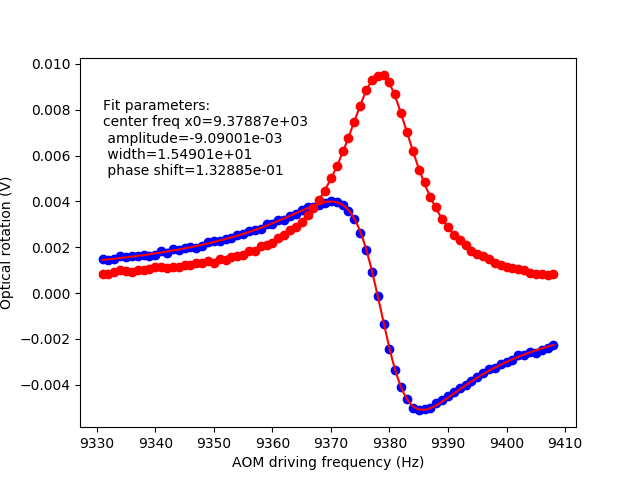
\includegraphics[width=0.4\linewidth]{figures/FM_NMOR}
\caption{Optical rotation vs. forced oscillation frequency...{\bf with
    a set of otherwise unknown parameters being used.  Also this
    figure is never referred to in the text, apparently.}}
\end{figure}

% Refer to appropriate Section of Chapter 2, if you want to make this
% statement.

%The quadrature components arise because exactly on resonance, the
%aligned atoms produce maximum optical rotation when the alignment
%axis is at an angle of $ \pi/4$ to the direction of the light
%polarization.

%Study NMOR signal by sweeping resonance frequency with amplitude
%modulated light.

%The magnetometer can be run as a forced oscillator, where a frequency
%generator is used to sweep the frequency of the laser amplitude
%modulator through the NMOR resonance. In this case the applied
%magnetic field~($B_z$) remains fixed during a measurement cycle
%(pumping and probing).
%The experimental setup for this measurement
%scheme remains almost same as for AM NMOR.

{\bf Fig.~\ref{fig:FMOR} shows something, but I do not know what.
  Below is my best guess as to what is displayed in
  Fig.~\ref{fig:FMOR}.}

\begin{figure}[h]
\centering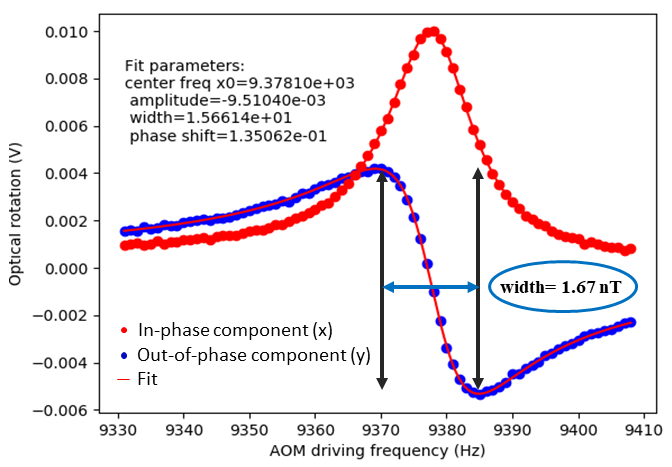
\includegraphics[width=0.5\linewidth]{figures/FM_modulation}
\caption{Demodulated components of the optical rotation, as a function
  of the forced-oscillation frequency.  NMOR resonance recorded with
  the 5 cm natural Rubidium cell, square-wave $100\%$ modulation of 1
  duty cycle. The $X$ component {\bf does not quite} reaches its
  maximum and the y component {\bf does not quite} have its zero
  crossing at $\Omega_m=2\Omega_L$ {\bf because of $\phi$}.  In this
  case the measured resonance width is 1.67~nT {\bf when translated
    from a frequency into a magnetic field???  It says a frequency, in
    the figure?  Lines drawn on the figure apparently do not line up
    with anything, and are meant to distract the
    reader?  I recommend to fix this figure.}.\label{fig:FMOR}}
\end{figure} 

The applied magnetic field was about 1~$\mu$T directed along light
propagation direction.  {\bf I think that this sentence is true.}

The measurement was taken by driving an Agilent 33522A function
generator to different modulation frequencies in order to find the
resonance frequency of the given Rb oscillator. The modulation
waveform is a square wave with a duty cycle of 1\%. Since our pump
beam is linearly polarized, a modulation at 2$\Omega_{L}$ is necessary
because of the two fold symmetry of alignment state. The typical range
of drive frequency is 9.31 KHz to 9.409 kHz for 1~$\mu$T field. An
unmodulated linearly polarized probe beam is used to analyze the spin
response. While the magnetometer response was recorded with a lock-in
amplifier, which is connected to balanced photodiode output,
demodulating the signal at the drive frequency of the atomic
oscillator.

{\bf The new things that I think I learned from this paragraph:}
\begin{itemize}
\item The duty cycle of the pump beam was 1\%.
\item The range of drive frequencies used in Fig.~\ref{fig:FMOR} was
  9.31 kHz to 9.409 kHz.
\end{itemize}


The center of the resonance is used to determine the Larmor frequency
and hence the magnetic field.  Fig.~\ref{fig:FMOR} shows the resonance
scan where data was taken by setting a function generator to different
drive frequencies for the given atomic oscillator. During the scan
drive frequencies was working as reference frequencies of the lock-in
amplifier. The red and blue data points indicate x and y output
respectively. When the modulation frequency is twice the Larmor
frequency the x component reaches its maximum and the y component has
its zero crossing. In this force oscillation scan the measured
resonance width is 1.67 nT.

{\bf The new things that I think I learned from this paragraph:}
\begin{itemize}
\item The red and blue data points indicate x and y output
respectively.
\item Something in the width corresponds to 1.67 nT, but it is very
  unclear how.
\end{itemize}

The probe beam then analyzed by photodiode whose output was connected
to a digital-signal-processing lock-in amplifier. The lock-in is
connected to a computer via GPIB. The DAQ computer saves the lock-in
data in a Python program where the data can be analyzed. The idea of
the fitting algorithm is to generate a concatenated function, having
the absorptive part as the first part and the dispersive as the second
(directly connected to each other). The corresponding frequency values
are simply the frequency scan range for the absorptive part while the
frequency increments are added to the maximum frequency point of the
absorptive in order to obtain the frequency parts for the dispersive
curve. This results in the overall data for the frequency, which is
inserted into the fitting function.

{\bf The new things that I think I learned from this paragraph.}
\begin{itemize}
\item There is a fit being done.
\end{itemize}


The function of absorptive part can be expressed as:
\begin{equation}
\phi_y= \frac{A_0 (X-X_0 )\omega_0}{2(X-X_0 )^2+(\omega_0^2)/4}\cos\theta-\frac{\omega_0^2A_0}{(X-X_0 )^2+(\omega_0^2/4)}\sin\theta
\end{equation}
while the dispersive part of complex lorentzian is given by
\begin{equation}
\phi_x= \frac{A_0 (X-X_0 )\omega_0}{2(X-X_0 )^2+(\omega_0^2)/4}\sin\theta+\frac{\omega_0^2A_0}{(X-X_0 )^2+(\omega_0^2/4)}\cos\theta
\end{equation}
In this conjunction, $A_0$ represents the maximum of the purely
absorptive curve, $\omega_0$ the width of resonance (FWHM) and $x_0$
the center resonance frequency. Furthermore, x represents the
frequency values.  The overall fitting function in order to really fit
a complex lorentzian is given by (the phases in R(x) and D(x) are not
considered in the following equations, since they are varied
(sin/cos)).

{\bf What I think I am supposed to get from this discussion:}
\begin{itemize}
\item The fit functions being used.
\end{itemize}


\begin{equation}
F = R(x)^{'}~\theta(x \leq f_{max}) + D(x-f_{max})^{'}~\theta(x > f_{max})
\label{equation:fit funtion}
\end{equation}
Where 
\begin{equation}
R(x)^{'}=R(x) . \cos(\phi_0)~ + D(x) .\sin(\phi_0)
\end{equation}\\
and
\begin{equation}
R(x)^{'}=D(x) . \cos(\phi_0) - R(x) .\sin(\phi_0)
\end{equation}

Here, $\phi_0 $ represents the phase shift between the absorptive and dispersive parts. This phase shift $\phi_0$ appears due to the wrong settings of lock-in amplifier. The actual fitting function in~ Eq~ \ref{equation:fit funtion} includes a case
structure, as it is given by the Heaviside-like function $\phi(x)$. If $ (x \leq f_{max}) $ ,$\phi(x)$ becomes zero,
if $(x > f_{max})$, it is equal to one. The initial guesses for the least-square parameters are given
as:\\
\begin{itemize}
\item
Amplitude $A_0$: In order to get guess amplitude, Averaging the maximum of the absorptive and dispersive curve is done.
\item
Width $\omega_0$: A width of the resonance curve of 15 Hz is assumed.
value.
\item
Center frequency $x_0$: The maximum frequency value of the
absorptive curve is considered as a guess for the center frequency.
\item
Phase $\phi_0$: In order to get a guess for the phase, $ R =\sqrt (
X^2 + Y ^2)$ is calculated for each
X and Y data pair. The corresponding X and Y data pair which gives the maximum
R value is taken and the phase guess $\phi _0$  is calculated by $\phi _0 = arctan(Y_{max}=X_{max})$.
\end{itemize}
Advantages: In the force oscillation scan technique entire resonance curve is scanned which allow us to see if there is a pure resonance or the real resonance curve get destroyed by any other external influences. By mapping out the entire resonance curve, we can easily debug the problem because in this process we can repeatedly adjust the power of the pump and probe beam immediately after each scan. Since the output signal of the balanced photodiode is demodulated stepwise by the lock-in amplifier at the modulation frequency at each increment, small amounts of noise induce in this process which is the most advantageous point of this field measurement technique. \\
Disadvantages: The force oscillation scan is a quite slow process which is the main drawback of this measurement scheme.
For a scan range of some hundred Hz usually takes a few minutes with  waiting time of couple second. As a result the force oscillation scans are not directly sensitive to magnetic field drifts, occurring at time intervals which are shorter than the actual scan. Field drifts would cause a degradation of the precision of a swept oscillation scan.

%\subsection{Self oscillation mode}

% This should be in Chapter 2.

%In self-oscillation mode\cite{PhysRevA.62.043403}, the output signal
%of photodiode is fed back to AOM for amplitude modulation. In this
%case the output signal of polarimeter is modified to act as a square
%wave which drives the AOM directly. After setting the phase and gain
%of the feedback system properly, the system start to oscillates
%spontaneously at the Larmor frequency. In order to measure the
%oscillation frequency a frequency counter can be used in this mode. An
%online tracking of the oscillating signal is also possible.

%A customized circuit board, consisting of an analog voltage amplifier,
%a Schmitt trigger, and two metastable circuits, is used to process
%optical rotation.  {\bf No, it isn't.}

%Advantages: Being a quite fast process and having a high bandwidth are
%the main features of this self-oscillation scan. In order to get rapid
%update of the magnetic field the magnetometer can be operated in this
%mode.

%Disadvantages: Since feedback loop self-oscillate in the case of
%constructive interference, it will work only for the signal having a
%phase shift of integer multiple of $2\pi$. This additional phase shift
%might be resulting into slightly off-centered resonance. As a result,
%self-oscillation mode is more susceptible to systematic errors in
%field measurement.



\subsection{Free Indution Deecay(FID) }
\bigskip
\begin{itemize}
\item The magnetometer can also
be run in free induction decay mode,where Rb atoms inside the cell is excited once and afterwards the decaying processes of the excited atoms is observed. A function generator is used to delivered the pump pulses which are necessary for pumping during a FID measurement. The output frequency of the function generator is set to the resonance frequency
\item Pumping is done for a very short time interval and the coherence decay takes place fast. The pumping process is instantaneously stopped by AOM (by applying a digital TTL signal an acousto-optic modulator can be used to shutter a laser beam on and off), which can also be used to trigger the  data acquisition (DAQ). 
\item The change in the optical rotation of probe beam is measured by balanced  photodiode and the output signal of the photodiode is then fed into the lock-in amplifier.
\item The reference signal on the lock-in amplifier has further to be set slightly off resonance ($\sim 100$ Hz) in internal frequency mode in order to properly record the FID.
The X and Y channels output of the lock-in amplifier are further transfered to a Tektronix oscilloscope. A python script is used to transfer the data presented on the oscilloscope screen to computer for further analysis. 
\end{itemize}
The entire process of pumpimg and probing during a measurement cycle in FID mode  has shown in Figure 4.2. Rb atoms are pumped using amplitude modulated laser beam for 0.1 sec and then observed the spontaneous decay of excited atoms for another 0.2 sec while the pump beam was off. \\
Table 4.1 shows the function generator and lock-in amplifier settings for FID measurement.
\begin{table}[h]
\centering
\begin{tabular}{|l |l|}
\hline

\textbf{ SETTING}    & \textbf{VALUE} \\
\hline
Function generator &   \\
\hline
Frequency & 9.4kHz   \\

Waveform    &  Square  \\

Amplitude   &  $1V_{pp}$  \\
Offset  &       500 mV  \\
Phase       &    $0\degree$ \\
Trigger     &   Manual  \\
Burst       &    1000 cycle \\
Amplitude modulation & On \\
\hline
Lock-in amplifier &     \\
\hline
Lock in frequency     & 9.297 KHz \\
Time constant     &  $300\mu s$ \\
Sensitivity      &  500mV  \\
\hline
\end{tabular}
\caption{Setting for FID at $1\mu T$ field\label{table:FID setting}}
\end{table}
\begin{figure}[h]
\centering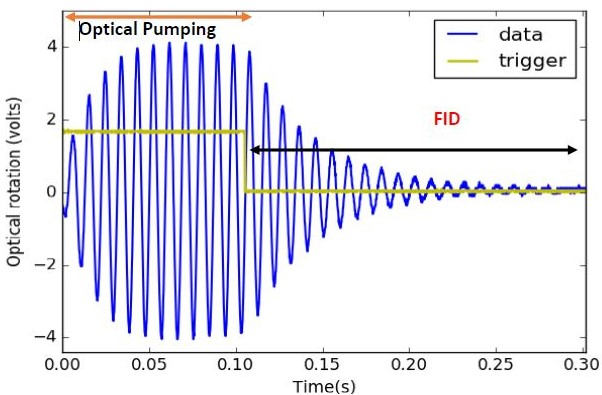
\includegraphics[width=0.55\linewidth]{figures/Capture2}
\caption{ An example of Free Induction Decay (FID) signal, when pumping the Rb atoms  was done for 0.1 s with linearly polarized light and probing was done for 0.2 s. The applied magnetic field during the measurement is $0.2~\mu T$. }
\end{figure}
The signal recorded  from X channel will be a sinusoid with an exponentially damping, according to   
  \begin{equation}
 y(t) = y_0 + A   e^{(t-t_0)/\tau}\sin(\omega t + \phi_0)\label{eq:decaying sinwave}
\end{equation}  

And the signal recorded  from Y channel will be a decaying cosine wave, according to
                                       
  \begin{equation}
 y(t) = y_0 + A   e^{(t-t_0)/\tau}\cos(\omega t + \phi_0)\label{eq:decaying coswave}
\end{equation}
where $y_0$ describes a possible offset, A is the maximum amplitude of the sinusoidal oscillation,
t the present time, $t_0$ the starting point of the measurement, $\omega$ the oscillation frequency and $\phi_0$  some possible phase shift. The data fitting procedure were done in two ways in order to study a variety of systematic effects that were encountered. One method is to take a least square fit of x and y data separately to a decaying sin and cosine wave respectively. Another way of data fitting is to fit X and Y data simultaneously. A least square-fit of the recorded data set to equation \ref{eq:decaying sinwave} or \ref{eq:decaying coswave} gives an estimate on frequency and  therefore the magnetic field.
\begin{figure}[h]
\centering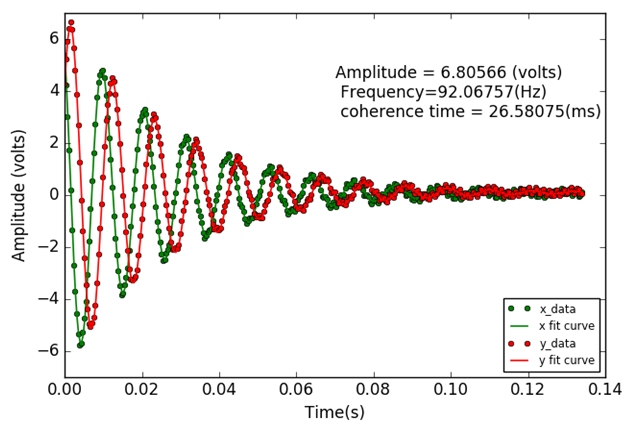
\includegraphics[width=0.55\linewidth]{figures/fid_simultaneous}
\caption{ Simultaneous fit of X and Y signal(green and red dots are represents x and y data respectively whereas green and red curve represents fit curves\label{Fig:FID fit}}
\end{figure}
  

The initial guesses for the least-square parameters are given
as:
\begin{itemize}
\item
Beat frequency $\omega$: In order to guess the beat frequency, the Fast Fourier Transform (FFT) of FID signal is done. The extracted FFT frequency is used as guess frequency.
\item
Amplitude A: In order to get guess amplitude, Averaging the maximum of the X and Y data is done.
\item
Offset $\phi_0$: The mean of FID signal is calculated. This mean value is used as guess for the offset. 

\end{itemize}
The data fitting procedure provides us the actual value for those parameters. The oscillation frequency, one of the extracted fit parameters, is then is used to estimate the magnetic field according to the following equation
\begin{equation}
 B= \frac{\nu_{fit}~ +~\nu_0}{2\gamma}\label{eq:field}
\end{equation}
 where $\nu_{fit}$ denotes the oscilation  frequency, $\nu_{0}$ is lock-in frequency and $\gamma$ is the gyromagnetic ratio of Rb vapor. Fig \ref{Fig:FID fit} shows an example least square fit of FID signal where both x and y output of lock-in has displayed.
 
Advantages: FID mode is free of  pump light induced frequency shifts or instabilities because the optical pumping is done for a very short time period and the frequency measurement takes place quickly. This frequency is later translate into magnetic field.\\ 

Disadvantages: As a finite duty cycle is used (pump modulation only happens during a short period of time and the main idea is to watch the coherence decay, a decreasing of the maximum achievable sensitivity with this method.



\subsection{FID in tilted magnetic field}
For the nEDM experiment it is very important to do tilted field measurement in order to have better understanding of  geometric phase effects which are the leading sources for systematic uncertainties during nEDM measurement . 
Since our Rb magnetometer is a scalar magnetometer, it is not possible to measure vector field components directly.In general, when the magnetic field is along the light propagation direction, the main resonance occurs at $\Omega_m = 2\Omega_L$. This resonance appear because of the symmetry of the optically pumped state. It is found that when magnetic field direction is tilted in the plane perpendicular to the light polarization axis, resonance is observed at  $\Omega_m = 2\Omega_L$~with its amplitude depending on the tilt angle. In this case, the amplitude of resonance signal decreases with increasing tilt angle . However, If we tilt the magnetic field direction towards the light polarization axis a new resonance appears at $\Omega_L$ along with the main resonance at $2\Omega_L$ if linearly polarized light is used. In this case the resonance signal contain two frequency component Fig \ref{fig:transverse} . The amplitude of the new resonance signal at $\Omega_L$  increases as the angle between B and the light propagation direction increases while main resonance amplitude at $2\Omega_L$  decrease with increasing tilt angle. However,when the tilt angle is larger than some certain angle the resonance amplitude measured at $\Omega_L$ also start to decrease and reaches zero when the magnetic field is directed along the y axis.   It could be possible to evaluate the magnitude of the magnetic field from the ratio of the resonance amplitudes at $\Omega_L$ and $2\Omega_L$. The same study with frequency modulated light has been reported by Pustelny et al.\cite{PhysRevA.74.063420}. In this study the NMOR Signal was observed by connecting the balanced photodiode to the oscilloscope directly. A python script is used to transfer the data presented on the oscilloscope screen to computer for further analysis. 

\begin{figure}
    \centering
 
    \begin{subfigure}[b]{0.45\textwidth}
        \centering
        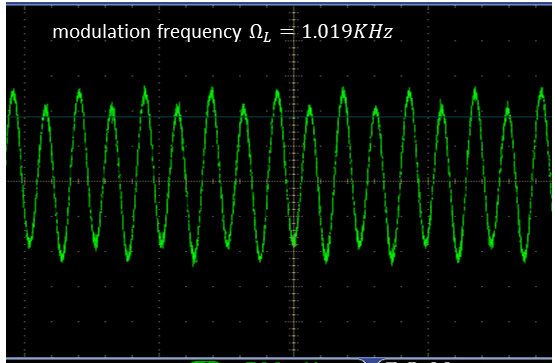
\includegraphics[width=\textwidth]{figures/transverse_field}
        \caption{}
        \label{fig:transverse}
    \end{subfigure}
    \hfill
    \begin{subfigure}[b]{0.45\textwidth}
        \centering
        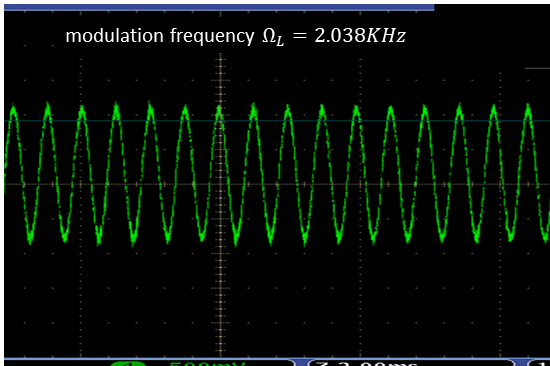
\includegraphics[width=\textwidth]{figures/transverse_field_2}
        \caption{}
        \label{fig:transverse2}
    \end{subfigure}
    \caption{(a) Optical rotation as a function of time at $\Omega_L$ in the yz plane at tilt angle $15\degree$ with light propagation direction. (b) Optical rotation as a function of time at $2\Omega_L$ for same tilt angle}
    \label{fig:Tilted field}
\end{figure}



% Chapter 5
\chapter{Experiments using the magnetometer\label{ch:results}}

In this Chapter I present the main results on measurements of the
properties of the magnetometer, optimization studies, and applications
of the magnetometer to characterize magnetic fields.  The main studies
that are presented are:
\begin{itemize}
\item Measurements of magnetic fields over long timescales using FID mode.
%  Conclusion: fields drift over time.  Question: how much is due to
%  magnetometer drift vs. other sources?
\item Adjustment of the pump and probe timescales in order to measure
  the field faster.
%  Allowed us to measure faster.
\item Magnetometer drift compared with drifts in the coil current and
  room temperature.  This study aimed at finding sources of drifts.
%Conclusion: neither drift seems
%  particularly correlated with field drift over long time periods.
%  Temperature stability seems quite good, consistent with Michi's
%  thesis.  Side conclusion: when field {\bf only} is changed, the
%  magnetometer responds as expected.  Implies that magnetometer works
%  well at sensing small changes in field, at least on shorter
%  timescales.
\item Studies of degaussing, which in part tell the story of our
  degaussing development and learning.  This includes studies of:
%with multiple goals, telling the story of
%  our degaussing
  \begin{itemize}
    \item the degaussing setup and testing it near zero field
%we set up the
%      system, we tested mainly sample rate (related to number of
%      oscillations) stated to be important in Thiel et al.  We found
%      that if the innermost shield was already degaussed that
%      additional poor/rapid degauss did not screw it up as badly as we
%      expected, until degaussing was very rapid.
    \item initial operations at non-zero field, and
%Ramp field to large values, without
%      degaussing was bad.  After degaussing was better.
    \item final degaussing procedure, in which degaussing the next to
      innermost shield was studied.
  \end{itemize}
\item Studies of laser locking and tuning, and the requirements on
  tune stability
%again multiple goals:
%  \begin{itemize}
%    \item Lock point or laser seems to drift over time.  See ``Drift
%      is about 120 pT'' where statistical error gets worse.  Also
%      would lose lock sometimes.  We think this may be due to PBS.
%    \item Other concern is whether drift of lock affects measured
%      field.  Studied by ``manual locking'' and found not to be
%      important.  Lock drift does not affect measured field drift very
%      much, but does affect statistical precision of magnetometer.
%  \end{itemize}
\item Studies pushing below 1~pT in an individual FID measurement.
  This includes adjustment of the pump and probe powers, and lock-in
  amplifier settings.  As will be shown, this study revealed problems
  in the procedures used to determine the precession frequency at such
  high precision and suggests avenues for further study.
%But when
%  we improved the statistical precision significantly, we began to run
%  into systematic errors in frequency measurement.  This led us to
%  study additional errors related to lock-in amplifier settings.
%  Future work is to finalize these studies in order to further reduce
%  the errors
\item Finally, I show my studies which revealed a way to use FID mode
  to measure transverse fields.
%Further work is
%  required to push to nT-scale transverse fields relevant for
%  typ.~unmeasurable gradients that enter $\delta_T$ correction in Hg-n
%  signals in nEDM experiments.
\end{itemize}
Each study will now be presented in turn and conclusions will be
summarized in Chapter~\ref{ch:conclusion}.

% Belongs in Magnetometer Literature Review Chapter 2?

%. In the case of AM NMOR, high-field
%resonance occur in addition to the regular zero-field resonance. The
%optical properties of the medium are being modulated at twice the
%Larmor frequency. In the case of strong external magnetic field, the
%dynamic Stark effect limits the sensitivity of NMOR based atomic
%magnetometry by reducing the accuracy of the field measurement. The
%advantage of using AM NMOR method is that it can reduce the Stark
%effect because light frequency is not affected by amplitude
%modulation\cite{gawlikoptical}. In AM NMOR, It is easily possible to
%control the number and amplitudes of the high field resonances by
%using the square wave modulation of light intensity.




\section{Long-term FID measurements\label{sec:long-term}}

A forced-oscillation scan or an acquisition of a single FID give a
measurement of the magnetic field within a relatively short time
period ($<1$~s).  For nEDM experiments, it is important to get
information about the change in the average magnetic field over time
periods of 100~s and longer.

In order to study the fluctuations and drifts in the magnetic field
over time, and to search for possible drifts in the magnetometer
itself, repeated measurements of FID's were made and recorded.

%long
%term data was taken in the FID mode.
During this long term process the laser frequency was tuned for
maximal FID amplitude, and locked using the DigiLock 110 module.  In
order to observe the FID signal, a Tektronix DPO 2014 oscilloscope was
connected to X and Y output of output of lock-in amplifier. A Python
script was used to set up the function generator and to trigger data
acquisition using the oscilloscope. The same script is also used to
transfer data continuously from oscilloscope to the computer.  For
further data analysis another Python script was used to process each
FID.  A least-squares fit was done for each FID for each X and Y pair.
The measured oscillation frequency of the decaying oscillating signal
was then convert to magnetic field using Equation~(\ref{eq:field}).

{\bf what are all the other settings of the magnetometer for these
  runs?  pump power is about 40$\mu$w,  pump time is 0.49~s,  probe power is about 22$\mu$w,  probe time is 0.5~s,  lock-in
  frequency is 1929.5 Hz , AOM frequency is 2038 Hz, lock-in time constant is 300$\mu$s...}

\begin{figure}%[h]
\centering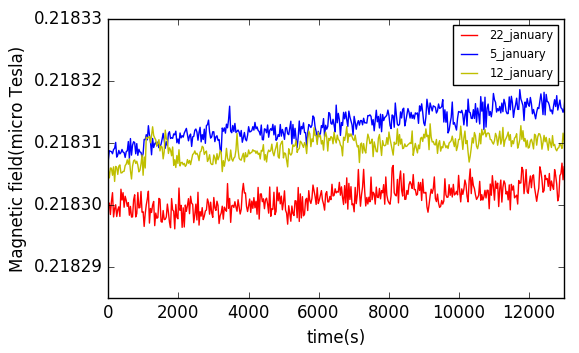
\includegraphics[width=0.85\linewidth]{figures/field_3_day}
\caption{Magnetic field recorded over 4 hours on three different
  days. The observed field drift is similar ($\sim 15$~pT) for each
  day.\label{fig:long-term-field}}
\end{figure}

Fig.~\ref{fig:long-term-field} shows the magnetic field recorded over
4 hours on three different days. Each data points in the graph
corresponds to a single FID measurement.  The observed field drift is
similar ($\sim 15$~pT) for each day.  The measurement was conducted at
0.2 $\mu$T magnetic field.

\begin{figure}%[h]
\centering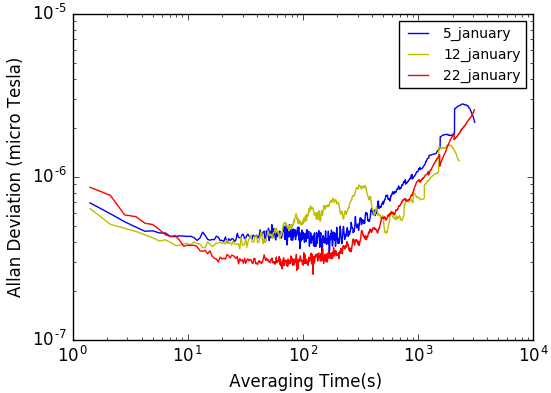
\includegraphics[width=0.8\linewidth]{figures/field_3_day_allan.png}
\caption{Allan deviation of recorded magnetic field vs.~averaging time
  for the time-series data presented in in
  Fig.~\ref{fig:long-term-field}.\label{fig:allan_deviation}}
\end{figure}

The Allan deviation was used to further quantify the long-term
stability~\cite{doe:website2} (see also Appendix~\ref{cite:appendix}.
Allan deviations characterize changes in the measured quantity when
the data are averaged on different timescales.  When the data behave
statistically on short timescales, the Allan deviation is equal to the
standard deviation.  If drifts occur, normally on longer timescales,
the Allan deviation grows linearly with a slope that $1/\sqrt{2}$
times the slope of the drift in time.

Fig.~\ref{fig:allan_deviation} shows the Allan deviations of the
measurements field presented in Fig.~\ref{fig:long-term-field}.  The
minimum in the Allan deviation occurs when statistical behavior is
overtaken by drift.  Fig.~\ref{fig:allan_deviation} shows that this
transition generally occurs after 10-60~s of averaging, corresponding
to a precision in magnetic field of 300-500~fT at the Allan minimum.

For an nEDM experiment, the goal precision is $\sim 20$~fT for the
average field over as measured over the 100~s neutron free-precession
measurement cycle.  This is not likely to be equivalent to the Allan
deviation minimum of our one magnetometer, because the long-term drift
is driven in part by the drift of the magnetic field within the
shield.  The goal of subsequent work was:
\begin{itemize}
\item to attempt to identify some of the sources of drift.  This
  included searching any sources that might be caused by the
  magnetometer itself, but also included the effects of
\item to improve the single FID performance so that fields could be
  measured faster.
\end{itemize}
In terms of the Allan deviation, it means trying to move the Allan
minimum lower and to the right.

\section{Optimization of cycle time} 

The goal of this optimization study was to reduce the cycle time
without sacrificing too much precision in the single-FID frequency
measurement.  If more measurements can be made more quickly, the
precision of the magnetometer over time would be improved.

\begin{figure}
\centering
\begin{subfigure}[b]{0.46\textwidth}
  \centering
  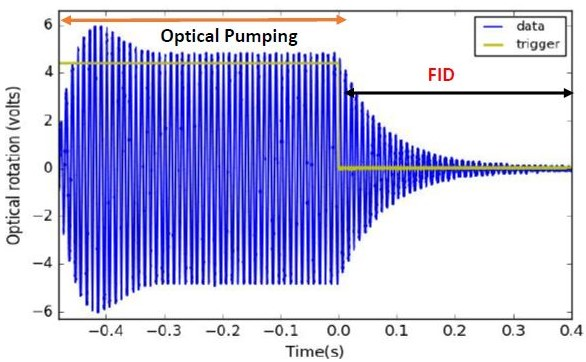
\includegraphics[width=\textwidth]{figures/Capture}
  \caption{}
  \label{fig:pump-long}
\end{subfigure}
\hfill
\begin{subfigure}[b]{0.45\textwidth}
  \centering
  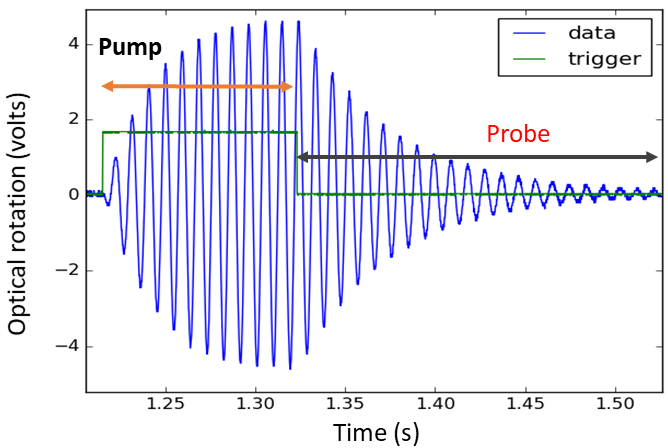
\includegraphics[width=\textwidth]{figures/FID_optimized.png}
  \caption{}
  \label{fig:pump-short}
\end{subfigure}
\caption{(a) FID signal for pump time 0.49~s and probe time 0.4~s. (b)
  FID signal for pump time 0.1~s and probe time 0.2~s.  Both
  measurements were conducted at $0.2~\mu$T magnetic field.}
    \label{fig:pump-time}
\end{figure} 


During this study the magnetometer was operated in FID mode at
0.2~$\mu$T field.
%A complete cycle of FID measurement consist of a
%pump time followed by a probe time.  Pump time represents the time
%atoms take to generate a polarized ground state. In this study we were
%trying to study how long the optical pumping of Rb atom should have
%continued in order to generate an alignment and optical pumping for
%long time does make any difference in measuring magnetic field
%precisely or not.
An example of our initial settings is shown in
Fig.~\ref{fig:pump-long}.  The pump time is 0.49~s and the probe time
is 0.4~s.  The amplitude of the differential photodiode signal is seen
to saturate well within 0.1~s.  The coherence time, indicated by the
decay time of the oscillating signal, is about 0.06~s.
Fig.~\ref{fig:pump-short} shows a more optimized the FID signal for
0.1~s pump time and 0.2~s probe time.

\begin{figure}%[h]
  \centering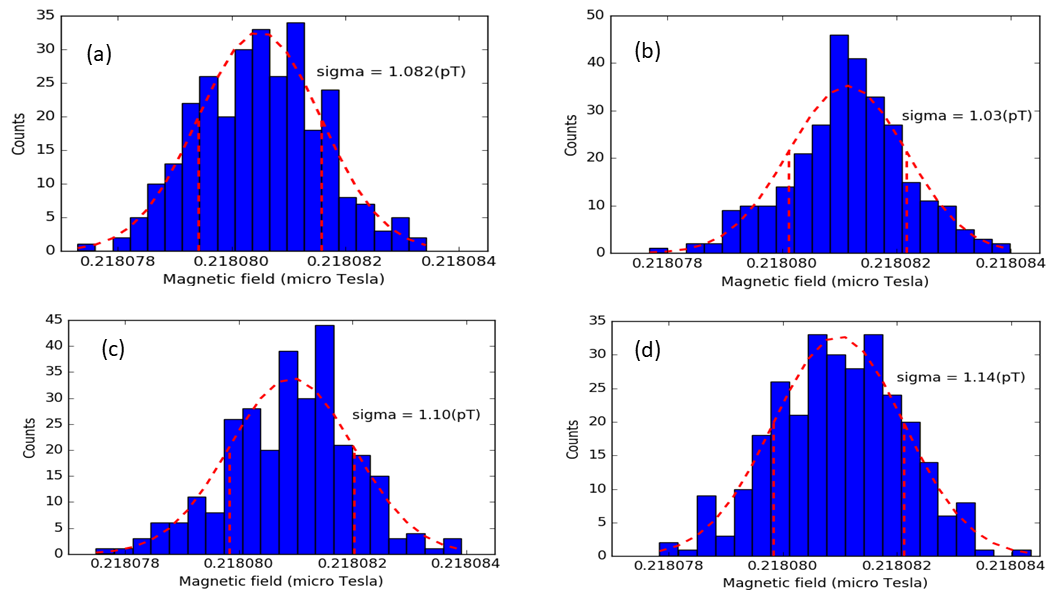
\includegraphics[width=0.75\linewidth]{figures/pump_time}
  \caption{Histograms of measured B-field for different pump times,
    {\bf for a measurement time of 300~s}. {\bf (a) is a pump time of
      0.49~s (b) is a pump time of 0.39~s (c) is a pump time of 0.2~s (d) is a
      pump time of 0.1~s.  The probe time in each case is 0.25~s.  The number
      of measurements taken in each case is therefore (a) 405 (b) 468
      (c) 666 (d) 857.  The standard deviation of each set of
      measurements is indicated in the respective
      figure.}\label{fig:different-pump-time}}
\end{figure}

In Fig.~\ref{fig:different-pump-time} a histogram of measured magnetic
fields by making subsequent measurements over 300~s is shown for
different pump times.  {\bf Which one is which? What is in the figure?
  The longer pump time is 0.49 s and the shorter one is 0.1 s.  What
  is the probe time.  How many measurements appear in each graph?}

From Fig.~\ref{fig:different-pump-time}, the pump time, when varied
over this limited range, does not strongly affect the precision of the
individual FID measurements.  {\bf However, it allows us to take
  measurements faster(It is possible to take 857 measurement in 300 s if cycle time is optimized to 0.35 s instead of 1 s.  How much faster?  You need to say the times
  and/or how many measurements.}
  
%  However for our Rb magnetometry setup the
%shortest pump time 0.1 s because 0.1 s is the minimum time atoms need
%to get aligned for making a coherence state after interacting with
%laser beam. Since the amplitude of FID NMOR signal reach it's maximum
%while atoms are in coherence state. Thus It is easy to understand
%coherence state is ready or not by observing the signal amplitude.

It is not surprising that the precision does not change much because
the amplitude of the differential photodiode signal during the pump
phase has saturated.

%In Fig.~\ref{fig:pump-long} the optical pumping is done for 0.49 s
%while signal amplitude reach its maximum over 0.1 s and after that
%signal amplitude remains unchanged till 0.49 s. In this case there is
%no point to pump more than 0.1 s. Same situation happens about probe
%time. If signal amplitude decays so quickly there is no point to set
%longer probe time. By optimizing pump and probe time we can speed up
%data acquisition system. After optimization for a single FID scan it
%only takes 0.35 s without losing any information. By using this faster
%data acquisition system it is possible to record multiple FID run with
%in a short period of time which is helpful to gather more information
%about magnetic field environment and helpful to achieve statistical
%precession.


\section{Magnet field compared with current in the $z$-coil}

\subsection{Field drift compared with current drift}

The idea was to determine the impact of possible current drifts.
  
An Agilent B2962A power supply was used to supply DC electrical
current to the $z$-coil.

\begin{figure}%[h]
\centering
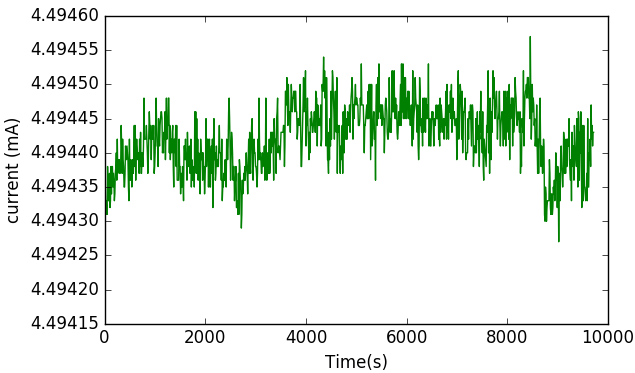
\includegraphics[width=0.6\linewidth]{figures/current}
\caption{Recorded current over 10000~s using Keithley multimeter %Agilent B2962A power source
{\bf How is this measured?  What is recorded by the power
    source?}.\label{fig:current} }
\end{figure}

Fig.~\ref{fig:current} shows the current {\bf measured how?} supplied
to the $z$-coil over a {\bf measurement} period of 10000~s.  The
current was set to 4.5~mA {\bf what is the correct value?  Was it set
  to 4.49440, or 4.494400, or 4.4944000 mA? 
  % current was set to 4.494400 mA
  If not, what is wrong
  with the power supply?} in order to achieve a magnetic field of
0.2~$\mu$T.  The maximum current excursion during the measurement
period was 30~nA.

\begin{figure}%[h]
\centering
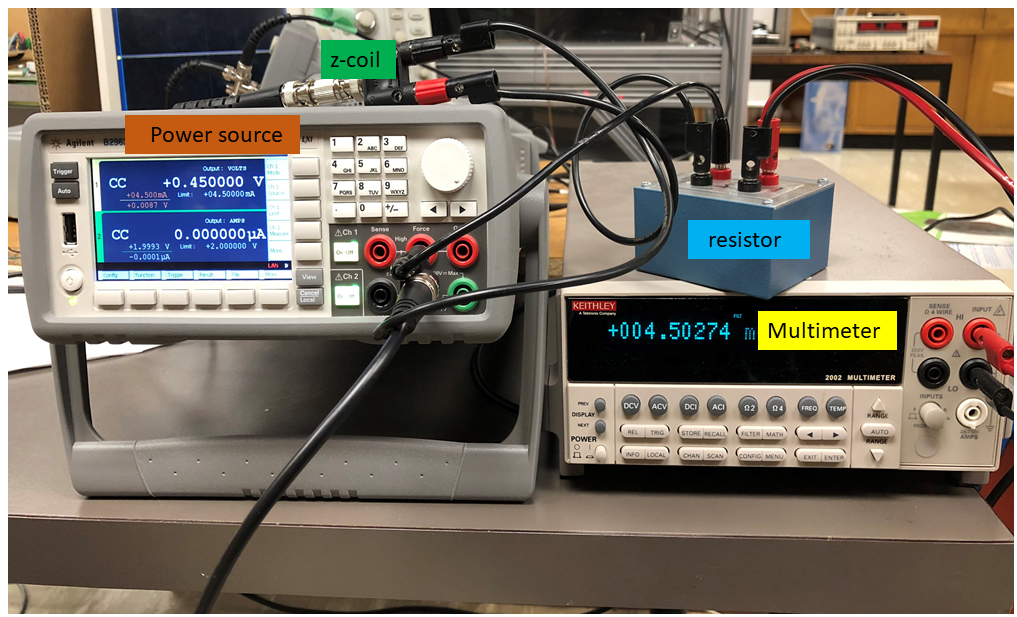
\includegraphics[width=0.6\linewidth]{figures/current_study_setup.png}
\caption{Arrangement for current stability study..\label{fig:Current_study_setup} }
\end{figure}


\begin{figure}
  \centering
  \begin{subfigure}[b]{0.67\textwidth}
    \centering
    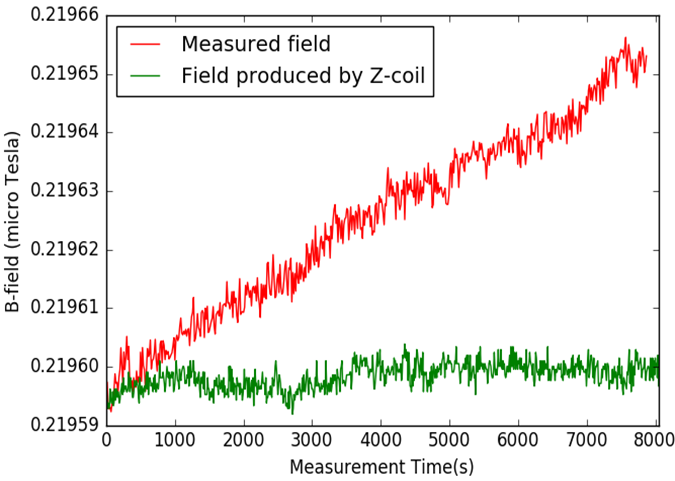
\includegraphics[width=\textwidth]{figures/field_coil_current.png}
    \caption{}
    \label{fig:field_measure_and_produced}
  \end{subfigure}
  \begin{subfigure}[b]{0.65\textwidth}
    \centering
    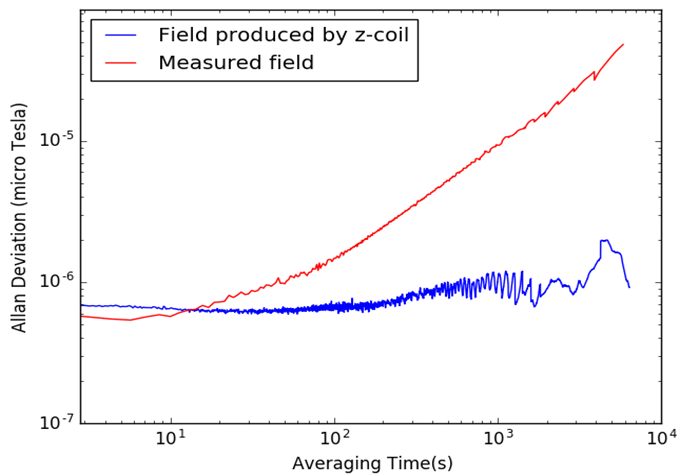
\includegraphics[width=\textwidth]{figures/field_current_allan_plot.png}
    \caption{}
    \label{fig:allan_plot}
  \end{subfigure}
  \caption{(a) Measured and produced magnetic field vs. time. {\bf
      what is each curve?}  (b) Allan deviation of field. {\bf why are
      the colors not the same as the above curves?  Why is the legend
      in the opposite order?}}
  \label{fig:current_vs_field_allan_deviation}
\end{figure} 

Fig.~\ref{fig:field_measure_and_produced} displays the magnetic field
measured by the magnetometer over the same period.  {\bf list all
  settings, lock-in time constant, laser power, lock-in frequency,
  magnetometer measured frequency, etc.}
%
produced by z-coil(green line) and measured field (red line) by
running the magnetometer in FID mode over 8000 s. The field generated
by z-coil is calculated by converting measured current to field with
coil constant of z-coil {\bf what value of the coil constant was used?
  According to my calcuation it is 0.048860236 uT/mA... this is not
  the same as the 48 nT/mA which you say it is...} (discussed in
Section~\ref{sec:internal-coil}). 
%yes you are right in this case I use the coil constant 0.04886025 uT/mA
At $t=0$ both fields {\bf are
  forced to?} coincide {\bf are normalized at t=0 by adjusting the
  coil constant to be XXX?} but over time a linear drift can be seen
in measured field.  For better understanding of the stability of the
power supply, providing current to the $z$-coil, the Allan deviation
of the generated field and measured field has shown in
Fig.~\ref{fig:allan_plot}.  It can be seen from the figure that
current stability is better than typical measured field changes.

{\bf How is the coil current measured? 
%Coil current was measured by using a Keithley 2002 multimeter.
Why was the coil current
  measured for longer than the field?  Was the coil current averaged
  over the same time as each frequency measurement? 
  % yes averaging time is same for current and frequency.
  Why is the
  current noisier than the magnetometer for short averaging times in
  the Allan deviation? 
  
  How were the current and field data acquired?
  How were the data synchronized to one another in time?  How is the
  measurement time defined for the coil current?  Is it at the start
  of the FID measurement or the end of the FID measurement, or
  somewhere in the middle, or asynchronously?  For the FID
  measurements, which time is graphed?  The start, end, or half-way
  time, or at the 1/e time of the FID?  Please show the measured coil
  current in the next section as well for
  Fig.~\ref{fig:field-change}.}



\subsection{Change in magnetic field driven by change in coil current}

A study has been conducted to determine the field change by changing
the coil current by a known amount. The main objective of this study
is to check the Rb magnetometer performance on magnetic field
measurement. During this measurement coil current has been changed by
$\pm~ 0.001$~mA. As a result a field change of $\pm$ 50~pT 
has been observed. The laser frequency was locked to Rb transition
frequency and all other setting kept unchanged. During this study the
magnetometer has been operated in FID mode {\bf list all documented
  settings.  What was the lock-in time constant, lock-in frequency?
  %lock-in frequency was 1950 Hz and time constant was 300 micro sec. AOM frequency 2049 hz, lock-in time constant 300\mu s.
  % probe power ~ 22 $\mu$W and Pump power~ 40 $\mu$W
  
  Were both x and y data simultaneously fitted? %only x data was fitted
  pump time?  probe
  time?%pump and probe time are 0.5 sec and 0.5 sec respectively.
  }.
\begin{figure}%[h]
\centering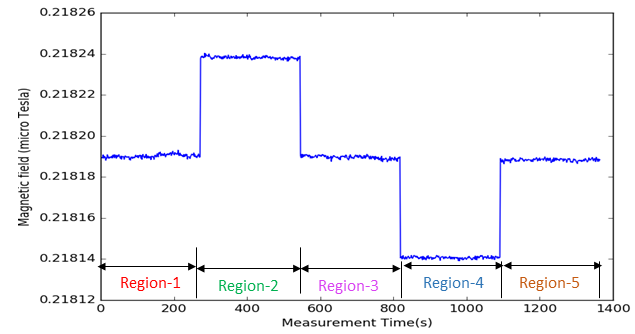
\includegraphics[width=0.7\linewidth]{figures/field_change_with_current}
  
\caption{The change in magnetic field  by changing coil current has been studied over 1400 sec. The blue line on different regions of the graph displays the measured magnetic field corresponding to the change in coil current. \label{fig:field-change}}
\end{figure} 
 
Fig.~\ref{fig:field-change} presents the magnetic field change over
time for different coil current. For better understanding
Fig.~\ref{fig:field-change} has been divide into five different
regions. In region-1 magnetic field has been recorded for 300 s while
the applied current to the Z coil was 4.5 mA {\bf do you mean
  4.500~mA?%  I mean 4.500~mA
  How many digits of precision are possible in the current
  supply? }%6.5-digit. 
  Then in region-2 the applied current to the z coil has
been increased by 0.0010 mA {\bf sig figs?} i.e., total current 4.5010
mA {\bf sig figs?} and measured the magnetic field for another 300
s. It is clear from the figure that the field has been changed
instantly by 50 pT due to the changed coil current. Now in
region-3, the coil current has been reduced to 4.5000 mA {\bf sig figs?}
and measured field for 300 s. After that the coil current has been
decreased by 0.0010 mA. As a result the field also decreased by
50~pT in this region.  Finally in region-5 the coil current has
 been set to 4.5000 mA again and observed the corresponing quick change in
field.

\section{Study the effect of room temperature in magnetic field} 

\begin{figure}%[h]
\centering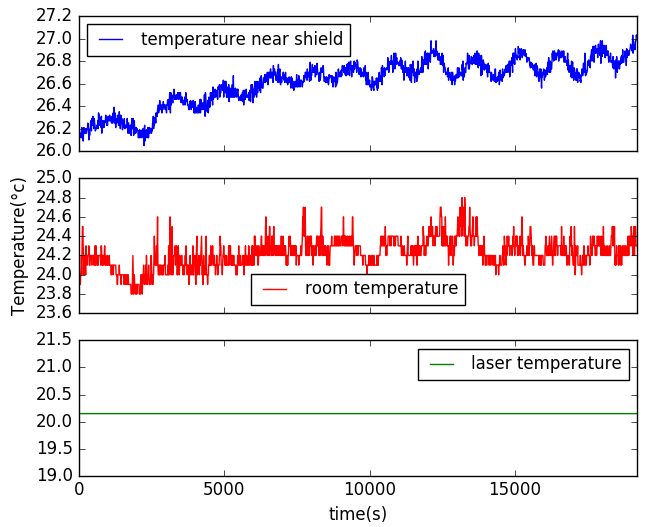
\includegraphics[width=0.8\linewidth]{figures/temp_.png}
\caption{Temperature measurement\label{fig:temperature-measurement}}
\end{figure}
Room temperature is measured using precision thermometer {\bf where?}
and laser temperature is measured from the output of the laser
temperature controller panel. The temperature on the magnetic
shielding {\bf where?  Why is it different than room temperature?
% I think the reason is that the optics table is fully covered by heavy curtains which make this place warmer than rest part of the room. I also discussed it with Dave he also mentioned me the same reason.
} is
measured by a T-type thermocouple.  Since T- type thermocouple is
non-magnetic we use this specific type of thermocouple instead of
K-type.
 
  \begin{figure}%[h]
\centering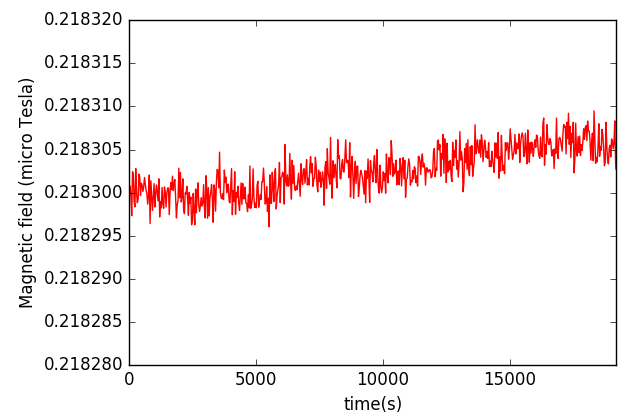
\includegraphics[width=0.8\linewidth]{figures/field_.png}
\caption{Field measurement\label{fig:field}}
\end{figure}

Fig.~\ref{fig:temperature-measurement} display the measured
temperature vs time.  During the measurement the laser temperature
(green line) remain unchanged which provide an indication about well
controlled laser diode temperature.  It can be seen from the figure
that room temperature fluctuation is 1\degree while temperature
outside of the magnetic shielding is about 0.8\degree.
Fig.\ref{fig:field} shows the magnetic field {\bf state all
  magnetometer settings}
  % probe power ~ 22 $\mu$W and Pump power~ 40 $\mu$W
  % lock-in frequency 1929.5 hz and AOM frequency 2036 hz, lock-in time constant 300\mu s.
  vs.~time while the temperature measurement
has taken place. In order to understand the correlation between
temperature change and field change, the measured field
vs. temperature has shown in Fig.~\ref{fig:field_vs_temp}. {\bf What
  was the data acquisition system for each device?  How were the data
  synchronized?% For room temperature measurement a precision thermometer was connected to a Agilent 34410A/11A 6 ½ Digit Multimeter. A python script was used to configures the multimeter for a 2-wire RTD measurement, triggers the meter, and then transfers the reading to the computer via instrument output buffer. And for temperature measurement near shield  the T-type thermocouple was connected with a Arduino Uno. For configuring this device and then transferring the reading to the computer a python script was used. 
  }  It is clear from the graph that there is no obvious
of field drift dependency on temperature.
  
\begin{figure}%[h]
\centering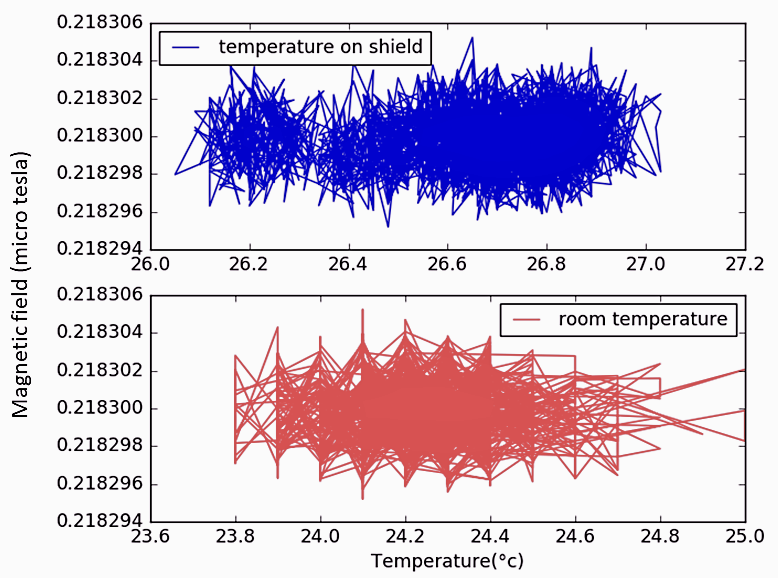
\includegraphics[width=0.6\linewidth]{figures/field_vs_temp.png}
\caption{Field vs. temperature\label{fig:field_vs_temp}}
\end{figure}
 
   
\section{Degaussing studies\label{sec:degaussing}}

\subsection{Initial tests using the magnetometer near zero field}

%different degaussing schemes(changing sample rate)
   
  
%Degaussing process is done in order to avoid the environmental
%perturbation and reduce any remnant field inside the four layer $\mu$
%metal magnetic shield \cite{doi:10.1063/1.2713433}. The setting for
%degaussing has shown in Table \ref{table:degaussing-setting}.  A
%detailed analysis of NMOR signal by changing the degaussing parameter
%could give us some information about the goodness of degaussing
%procedure. Toward this end, a study has been carried out to determine
%the dependency of the resonance width on the sample rate (see
%discussion on section \ref{sec:Degaussing}).

We used the procedure described in Section~\ref{sec:near zero field}.  To
remind the reading, the procedure is:
\begin{itemize}
\item Initiate the degaussing sequence in one channel of the function
  generator.
\item Once complete, ramp the rheostat to zero and open the switch.
\item Pressing a button on the computer initiates the ramp of the
  $z$-coil on the second channel of the function generator, which
  calibrates the optical rotation to field.
\item Both the current in the $z$-coil and the differential photodiode
  signal are monitored at all times using an oscillscope.
\end{itemize}

%In this study, data was acquired by sweeping the magnetic field near zero field. Before each measurement degaussing the innermost layer of shield has done. During this measurement only one degaussing parameter, sample rate, was varied in order to study the effect of degaussing parameter on magnetic field measurement.  

\begin{figure}%[h]
  \centering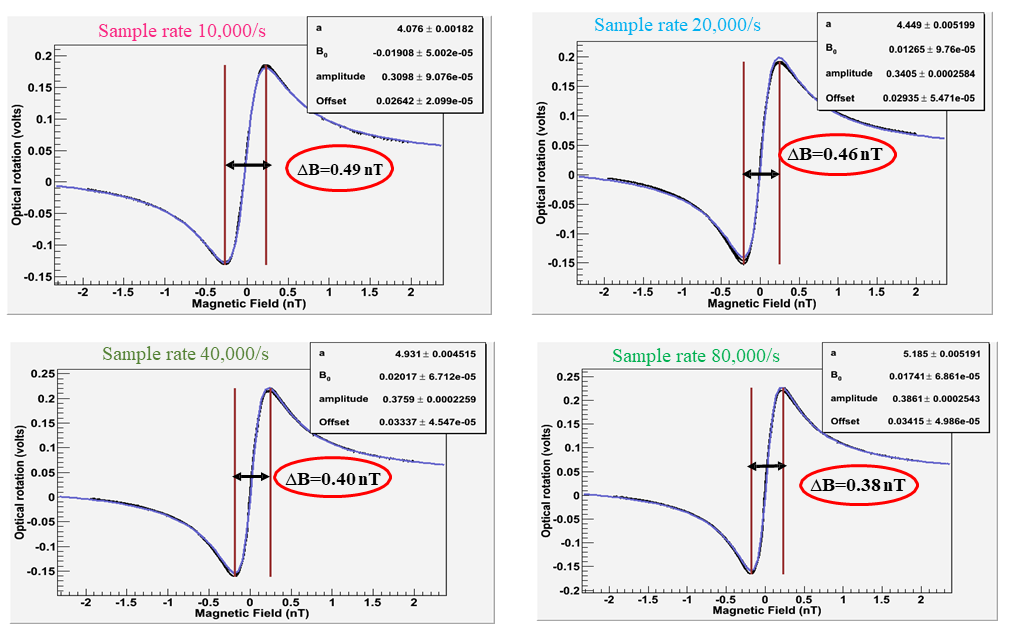
\includegraphics[width=\linewidth]{figures/sample_rate}
  \caption{ Optical rotation vs. measured B-field for different sample
    rate.  {\bf What order were the data taken in?% smaller sample rate to higher sample rate
    }  The numbers
    written in the red circles indicate the distance in magnetic field
    from the optical rotation minimum to the optical rotation maximum
    $\Delta B$, as deduced from the fit parameter $a$.  The fit
    parameter $B_0$ indicates the remnant field sensed by the
    horizontal offset of the dispersive shape, reported in
    nT.\label{fig:different-sample-rate}}
\end{figure}

Optical rotation as a function of magnetic field for different sample
rate has shown in Fig.~\ref{fig:different-sample-rate}.  Recall that
the sample rate determines the rapidity with which the $5\times 10^5$
individual samples of the linear degaussing envelope function are
stepped through.  A sample rate of 10,000/s therefore represents a
degaussing time of 50~s.  Since the carrier wave in all cases is
10~Hz, it means that 500~cycles were used.  The sample rate of
80,000/s represents a degaussing time of 6.25~s and 62.5 cycles.

It should also be noted that the data were acquired in order of
increasing sample rate, and that many additional degaussing sequences
were conducted which are not shown in
Fig.~\ref{fig:different-sample-rate}.

We had expected that larger sample rate would manifest itself as a
worse degaussing resulting possibly in worse magnetometer performance.q
Paradoxically, the resonance width $\Delta B$, the difference between
two peak of the dispersive curve, reduced as the sample rate was
increased.  It can be seen from Fig~\ref{fig:different-sample-rate}
that, the resonance width is about 0.49~nT for sample rate 10,000/s
and the resonance width is 0.38~nT for sample rate 80,000/s.  This is
likely an indication of a small change in the transverse fields or
generally an improvement the homogeneity of the field.  This is
consistent with the observation that the amplitude grows slightly with
amplitude, which is another indication of the field quality, all other
magnetometer settings being equal.

The remnant field $B_0$ is an indication of the average longitudinal
field (along the laser beam axis) and is within 20~pT of zero.  It
increased with the sample rate from a starting negative value to a
positive value.

The conclusion of this study was that additional degaussing, as long
as it has a reasonable number of cycles, tends not to affect the field
or to improve slightly the homogeneity of the field.  Generally the
field is always reduced below 20~pT.

%\begin{figure}%[h]
%\centering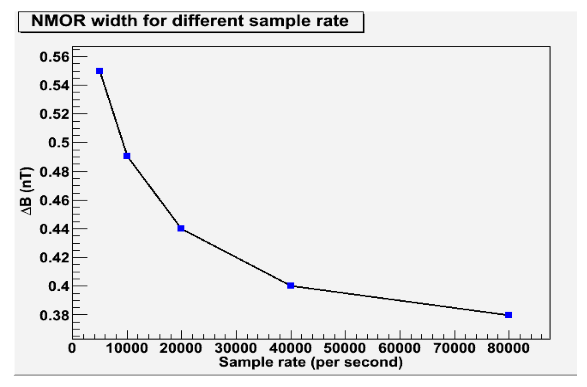
\includegraphics[width=0.6\linewidth]{figures/field_vs_sample_rate}
%\caption{Resonance width vs.~sample rate. Resonance width decreases
%  with increasing sample rate.  When the sample rate is 5000~samples/s
%  the observed resonance width is 0.55~nT. On the other hand the
%  resonance width is 0.38~nT for sample rate 80000
%  sample/s. \label{fig:resonance width vs. sample rate} }
%\end{figure}

%Fig~\ref{fig:resonance width vs. sample rate} shows the resonance
%width as a function of sample rate. Resonance width decreases with
%increasing sample rate.  It is obvious from the graph that the
%resonance width becomes narrower for larger sample rate.

\subsection{Measurements at 0.2~$\mu$T and initial studies of the effect of degaussing on field stability\label{sec:three-degauss}}
%Ramp field up/down 

The previous results implied that additional (even poor) degaussing
had little impact if the previous degaussing was done adequately.  To
address this, we began to do studies where the internal $z$-coil field
was purposely ramped to a large value, then reset to a low value for
measurements at non-zero field.

%A study has conducted by making the magnetic field environment bad
%inside the shielding intentionally by ramping the field from a lower
%value to higher value and observe any change in field drift. This
%study has done in 3-steps:
%  \begin{itemize}
%      \item take field measurement for about 2000 s without performing any degaussing.
%      \item Intentionally make the field environment bad and take field measurement for another 2000 s. No degaussing has done in this step also.
%      \item perform degaussing of the innermost shield and again measured magnetic field for 2000 s.
%  \end{itemize}

\begin{figure}
  \centering
  \begin{subfigure}[b]{0.425\textwidth}
    \centering
    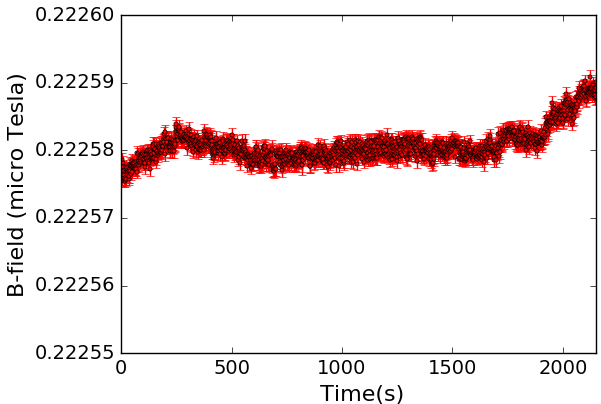
\includegraphics[width=\textwidth]{figures/ramp_1}
    \caption{}
    \label{fig:ramp-up}
  \end{subfigure}
  \hfill
  \begin{subfigure}[b]{0.42\textwidth}
    \centering
    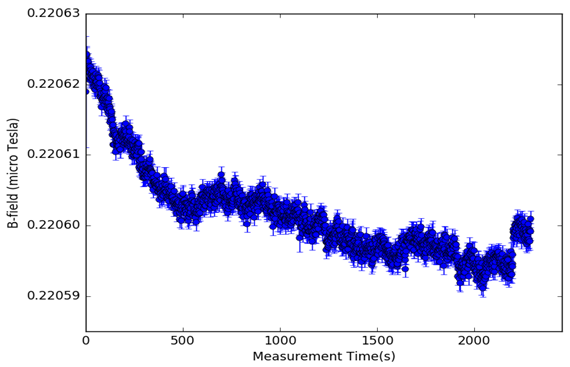
\includegraphics[width=\textwidth]{figures/ramp_2}
    \caption{}
    \label{fig:ramp-down}
  \end{subfigure}
  \begin{subfigure}[b]{0.42\textwidth}
    \centering
    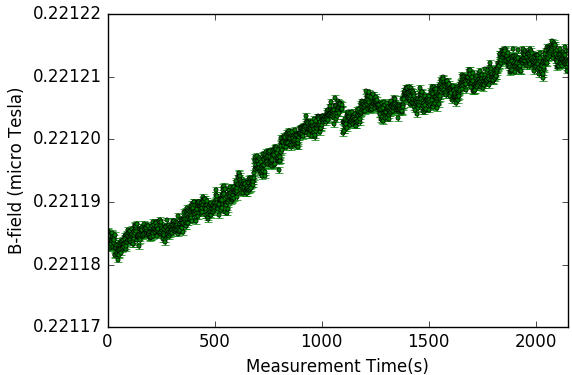
\includegraphics[width=\textwidth]{figures/ramp3}
    \caption{}
    \label{fig:degauss}
  \end{subfigure}
  \caption{Measurements conducted in time order from (a) to (b) to (c)
    under different degaussing conditions at $B_z=0.2~\mu$T magnetic
    field: (a) no degaussing, (b) ramp $B_z$ from 0.2~$\mu$T to
    10~$\mu$T then again set it to 0.2~$\mu$T and collect FID signal
    before degaussing, and (c) after degaussing.}
  \label{fig:ramp-updown}
\end{figure}

Fig.~\ref{fig:ramp-updown} shows an example of such a study.  In all
three cases shown in Fig.~\ref{fig:ramp-updown}, the magnetometer
settings are similar.  Since the field changed in each measurement,
the magnetometer was retuned each time, principally the pump frequency
and the lock-in amplifier internal reference frequency.  {\bf What are
  the magnetometer settings?}
 % AOM frequency 2064 Hz and lock-in frequency 1950.2 Hz (fig:5.12(a))
 % AOM frequency 2059 Hz and lock-in frequency 1950.2 Hz (fig:5.12(b))
 % AOM frequency 2078 Hz and lock-in frequency 1950.2 Hz (fig:5.12(c))
  

In the 1st part of this study the magnetometer was operated in FID
mode at 0.2~$\mu$T field, {\bf at a point in time when the
  magnetometer had been operated in a quiet environment for several
  days?}. The recorded magnetic field measurement over a 2200~s period
in this condition is shown in Fig.~\ref{fig:ramp-up}.  It can be seen
from Fig.~\ref{fig:ramp-up} that the magnetic field increased linearly
for first 300~s then showed a decrease in field. The field was pretty
stable between 600~s and 1800~s and after that the field showed an
increase. The overall field change is about 15 pT during the
measurement.  In Fig.~\ref{fig:ramp-down}, data was acquired by
ramping $B_z$ from 0.2~$\mu$T to 10~$\mu$T then down again to
0.2~$\mu$T and collect FID signal.  Since the $z$-coil is coupled to
the inner shield system, this should magnetize the shields.  By doing
this field ramping we intentionally perturb the magnetic field
environment inside the shield.  After this field ramping the long term
field measurement has been conducted for another 2200 s. In this case,
the field showed a downward drift of about 35~pT.  Thus field ramping
did seem to change the magnetic environment inside the magnetic
shielding.  Finally, for Fig.~\ref{fig:degauss}, the innermost
magnetic shield was degaussed {\bf with what sample rate, etc.?% the innermost shield was degaussed with degaussing parameters stated in Table \ref{table:degaussing-setting}
What
  procedure was followed?}. 
  % Before starting field measurement via FID mode degaussing was done multiple times (4-5 times) repeatedly. During the measurement no degaussing was done. 
  
  While this changed the direction of the
drift, it did not change the magnitude of the drift which was again
35~pT over 2200~s.  {\bf Is it true that no amount of degaussing of
  the innermost shield changed this significantly?}

During this time we began to develop a hypothesis about magnetic
couplings inside the magnetic shielding.  We realized that the
$z$-coil, which had been designed to be coupled to the innermost
shield, was now more strongly coupled to the second innermost shield.
This is because most of the flux in the solenoidal winding exits the
end of the innermost shield, whose endcaps have been removed in order
to accommodate its degaussing coil.


\subsection{Effect of degaussing second innermost and two other outer shields}
 
If the system had been kept at low field for several days, the usual
field drift was about 15 pT over 3000~s (as discussed in
Sections~\ref{sec:three-degauss} and~\ref{sec:long-term}).
After doing a transverse field study (applying current to $x$- and
$y$-coils along with $z$-coil, like that reported in
Sections~\ref{sec:ch4_tilted_field} and~\ref{sec:tilted-results}) the
magnetic field environment became even more unstable.

\begin{figure}
  \centering
  \begin{subfigure}[b]{0.45\textwidth}
    \centering
    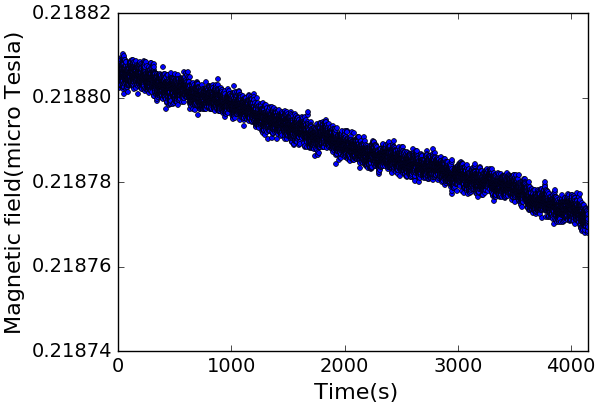
\includegraphics[width=\textwidth]{figures/before_degaussing}
    \caption{}
    \label{fig:without DG}
  \end{subfigure}
  \hfill
  \begin{subfigure}[b]{0.47\textwidth}
    \centering
    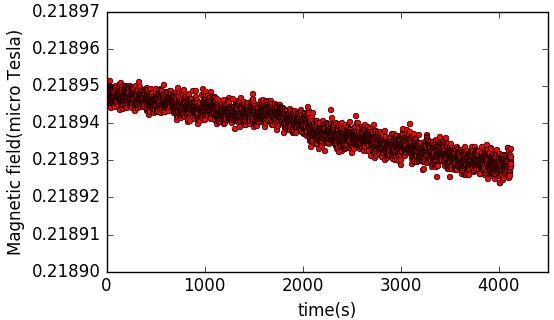
\includegraphics[width=\textwidth]{figures/innermost_degaussing.png}
    \caption{}
    \label{fig:with_DG_innermost}
  \end{subfigure}
  \begin{subfigure}[b]{0.45\textwidth}
    \centering
    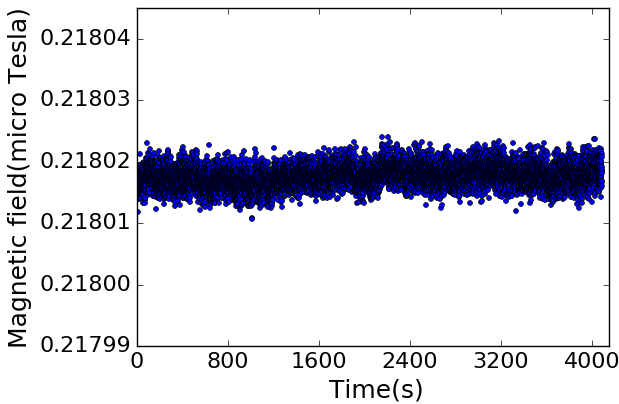
\includegraphics[width=\textwidth]{figures/after_degaussing}
    \caption{}
    \label{fig:with DG}
  \end{subfigure}
  \caption{Magnetic field recorded over 3 hours. (a) The stability of
    magnetic field without performing any degaussing. A downward field
    drift of about 45 pT was observed in this case.(b) Magnetic field as a function of time after degaussing the innermost shield. Still the field drift is about 30 pT.  (c) Magnetic field
    stability after degaussing the 2nd innermost layer of magnetic
    shielding. Only a couple pT field drift has observed in this case. During this study the signal amplitude was pretty
    low($\sim$3V) because of the low pump beam power(I think) or other poor settings. As a result the precession width becomes wider(10~pT)
  while the usual is about 5~p
    \label{fig:effect of DG}}
\end{figure}

Fig.~\ref{fig:without DG} shows about 50~pT drift in magnetic field in
4000~s.  In order to cancel background field inside shield degaussing
innermost layer of mu-metal is done but it doesn't help to solve field
drift problem (\ref{fig:with_DG_innermost}){\bf where is this data?}. During those three measurement {\bf which
  study? the one ``without performing any degaussing'' as written in
  the figure caption, or after degaussing the innermost shield?}  the
lock-in reference frequency is set to 1938.5~Hz and lock-in time
constant is 300~$\mu$s.  Then degaussing the 2nd innermost layer of
shield is done which solve the field drift problem (see Fig \ref{fig:with DG}){\bf where is this
  data?  Is this (b)?}% yes.

Since the end cap of the innermost shield layer is not in use some
background field leaked into 2nd layer which was causing the drift in
field. So by degaussing the 2nd layer of shield canceled background
field and field becomes so stable (Fig.~\ref{fig:with DG}). During this
three measurement all other setting remain unchanged only the degaussing
of the 1st and 2nd innermost shield has performed.
   
%   \end{itemize}
  
\section{Laser tuning} 
\begin{itemize}
\item effect of careful tuning

The main purpose of this study is to understand the importance of
laser tuning on coherence life time of excited atoms. During the study
optical pumping is done to polarize the rubidium atom and hence
produce coherence state. When the laser light is exactly tuned to
resonance with the atomic transition, the lifetime of coherence state
becomes longer and the amplitude of resonance signal reaches its
maximum. On the other hand coherence state decay quickly when laser
frequency detunes from atomic transition. In this case, the signal
amplitude reduces due to frequency detuning.

\begin{figure}
  \centering
  \begin{subfigure}[b]{0.45\textwidth}
    \centering
    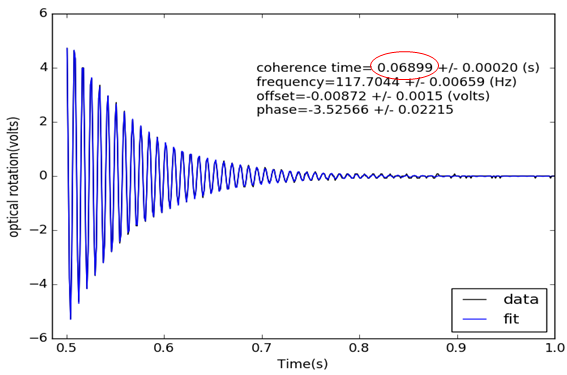
\includegraphics[width=\textwidth]{figures/perfect_tuning}
    \caption{}
    \label{fig:good tuning}
  \end{subfigure}
  \hfill
  \begin{subfigure}[b]{0.45\textwidth}
    \centering
    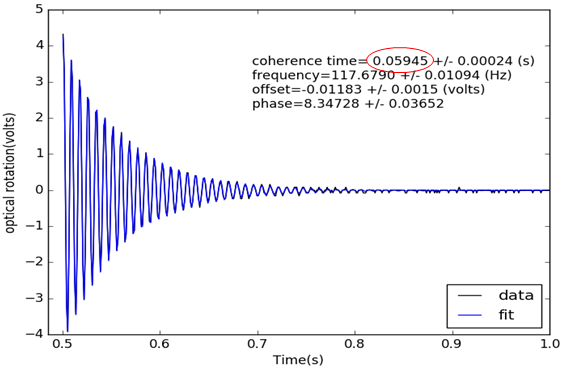
\includegraphics[width=\textwidth]{figures/bad_tuning}
    \caption{}
    \label{fig:bad tuning}
  \end{subfigure}
  \caption{(a) Recorded FID signal while laser is perfectly tuned to
    atomic transition frequency. (b) FID resonance signal when laser
    is slightly {\bf quantify} detuned from transition frequency.}
  \label{fig:effect of tuning}
\end{figure}
	
Fig~ \ref{fig:effect of tuning} shows the effect of laser tuning on
coherence lifetime. During this measurement the AOM frequency was set
to 2.068~kHz and Lock-in frequency was 1.950~kHz.  For proper {\bf
  what does ``proper'' mean?  How proper is proper?}  laser tuning the
observed coherence time is 68 ms (Fig \ref{fig:good tuning}) whereas
for bad tuning {\bf what does ``bad'' mean in this case?  How bad is
  bad?}  coherence time reduces to 59 ms (Fig \ref{fig:bad
  tuning}). On a fundamental level, the magnetometer actually measures
the energy splitting between the Zeeman sublevels of the atomic ground
state due to the magnetic field. The linewidth of such a spectroscopic
measurement is given by the coherence lifetime $T_2$ of the atomic
spins \cite{bib:Seltzer_thesis}
\begin{equation}
 \Delta B = \Delta\omega/\gamma  = 1/γ T_2
\end{equation}

The development of a sensitive magnetometer depends on achieving the
maximum possible polarization lifetime.  For very short coherence time
atomic spin depolarize quickly which limits the sensitivity of the
magnetometer.  Since longer coherence time and larger signal amplitude
indicate better frequency precession and therefore precise field
measurement it is very important to make sure the laser tuning has
done carefully.

{\bf I do not understand the above item at all.  There is no
  indication of what good or bad means.  There is no indication of
  even the scale of the detuning.  I have no idea how to learn
  anything from this section and I don't understand the point of it.}


\item problem with drift of tune {\bf this will turn out to be a bad
  title for this bullet}\\
  \begin{figure}%[h]
    \centering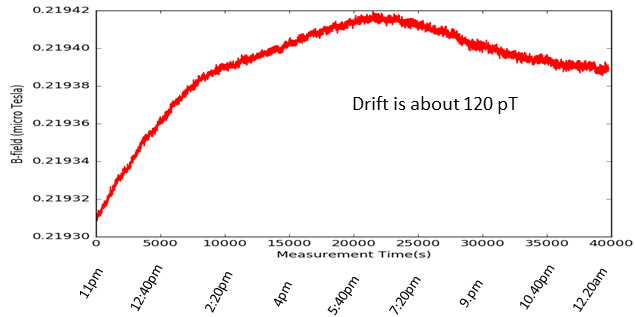
\includegraphics[width=0.6\linewidth]{figures/field_drift}
    \caption{Magnetic field recorded over 12~hours.  In this
      measurement the observed field drift is
      about~120~pT.\label{fig:digilock-drift}}
  \end{figure}
  For studying long term stability data was taken for about
  12~hours. Laser was locked using the DAVLL system described in
  Section~\ref{sec:DAVLL}. Fig \ref{fig:digilock-drift} shows 120~pT
  observed drift in magnetic field over 12~hours. Although DAVLL was
  in use laser frequency was not locked for 12~hours {\bf it was
    locked.  It's just that the lock-point was changing, we think.
    What you mean is that the frequency was drifting.  The reason we
    {\it think} or {\it suspect} that it was drifting is because the
    error bar is increasing.  Strangely, you do not mention this.}. As
  a result laser tuning moved due to mode hoping which causes the
  drift {\bf I have never seen any evidence of this.  What is the
    evidence?}. The current laser locking system only works perfectly
  for maximum 4 hours {\bf Please show the data that proves this}. The
  possible reason for this mode hoping is the Polarizing beam
  splitting cube of our DAVLL system~\cite{principles}. The
  disadvantage of using this type of PBS is that they show flaky
  optical behavior over longer times\cite{bib:Philip2008}.
  %{\bf please provide a citation for this statement}.

  {\bf Again, I do not understand this section.  A bunch of statements
    are made with only one graph showing that the drift in the field
    is 120~pT.  Where is all the evidence for the other statements?}

  {\bf The only point to made here is that the statistical error in
    the data gets bigger over time and we think hey, maybe that's due
    to the laser tune drifting.  Do we know that at this point?  No,
    because there is absolutely no data that you have shown that
    demonstrates it.  This is called a ``hypothesis''.  I think in the
    next section, you are testing that hypothesis.}

  {\bf If there is any other data that would substantiate your
    statements, please present it.}
  
\item manual tuning

During this study frequency of laser light was tuned to atomic
transition maximize optical rotation. The DAVLL and Digilock system
was not used to lock the laser.  Rather, periodically, the data
acquisition was paused, and the laser frequency was adjusted manually
to maintain the same (largest) different photodiode amplitude. The
data acquisition would then be restarted.

\begin{figure}
  \centering
  \begin{subfigure}[b]{0.45\textwidth}
    \centering
    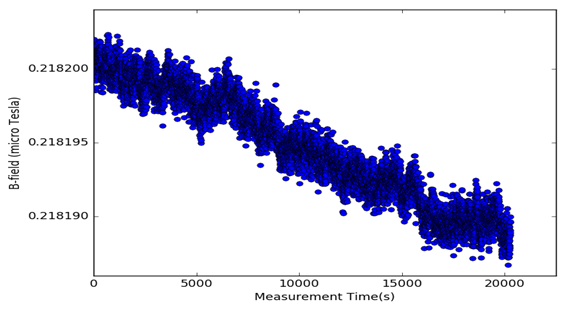
\includegraphics[width=\textwidth]{figures/manual_tuning}
    \caption{}
    \label{fig:field-manual-tuning}
  \end{subfigure}
  \hfill
  \begin{subfigure}[b]{0.45\textwidth}
    \centering
    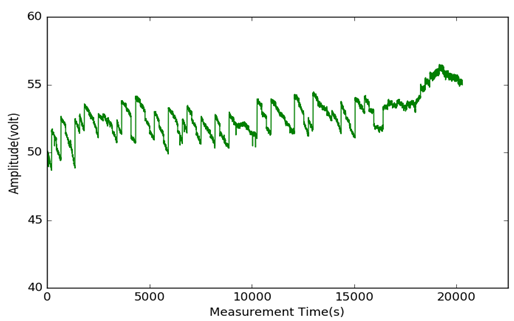
\includegraphics[width=\textwidth]{figures/amplitude_manual_tuning}
    \caption{}
    \label{fig:amplitude-manual-tuning}
  \end{subfigure}
  \caption{(a) magnetic field vs. time. (b) {\bf The vertical scale
      appears to be labeled incorrectly (units)} amplitude of recorded
    FID NMOR signal over 20000~s. During this study laser tuning is
    maintained manually, as can be seen from the jumps in the
    amplitude which occur upon retuning.}
  \label{fig:manual-tuning}
\end{figure}
   
The results of the measurement are shown in
Fig.~\ref{fig:manual-tuning}.  Fig.~\ref{fig:amplitude-manual-tuning}
shows the fitted initial amplitude (after the pump beam has been
switched off) as determined by the fit to the decaying oscillating
function.  The spikes in Fig.~\ref{fig:amplitude-manual-tuning}
indicate times when the retuning of the laser was conducted, as
described above.

Fig.~\ref{fig:field-manual-tuning} shows the result of the frequency
measurement, when translated into magnetic field.  It can be seen that
as the amplitude of the fit decreases (presumably due to a drift in
the laser frequency), the statistical fluctuations in the field
measurement increase.  This would be expected because a small fit
amplitude will make the frequency statistically more difficult to
measure.

Clearly the field measurement in Fig.~\ref{fig:field-manual-tuning}
does not drift in the same way as the amplitude in
Fig.~\ref{fig:amplitude-manual-tuning}.  Thus we conclude that the
field measurement in FID mode is relatively insensitive to the
frequency tuning of the laser, except that if the tune drifts, the
frequency measurement becomes statistically less precise.

%we can say that during this measurement the amplitude
%of FID NMOR was pretty stable except small fluctuations over 20000 s
%. The observed small fluctuation is due to the manual adjustment while
%keeping the laser frequency tuned to atomic transition over long
%period of time. Obtaining stable signal amplitude is a indication that
%laser is not drifting to much. Although laser frequency was not
%drifting a lot during the measurement, still there is a drift in
%magnetic field (Fig.~\ref{fig:manual-tuning}). The overall drift is
%about 20~pT over 20000~s. So it can be conclude that the drift in
%laser frequency is not the main reason behind this induced field
%drift.

\end{itemize}


\section{Improving the precision of individual FIDs, and problems encountered in doing so\label{sec:reference-frequency}}

\subsection{Optimization of pump and probe beam power} 
A study has been performed to determine how optimization of the pump
and probe beam power effect on precise field measurement.  During this
study, the magnetometer has operated in FID mode.
  \begin{figure}
    \centering
    \begin{subfigure}[b]{0.7\textwidth}
        \centering
        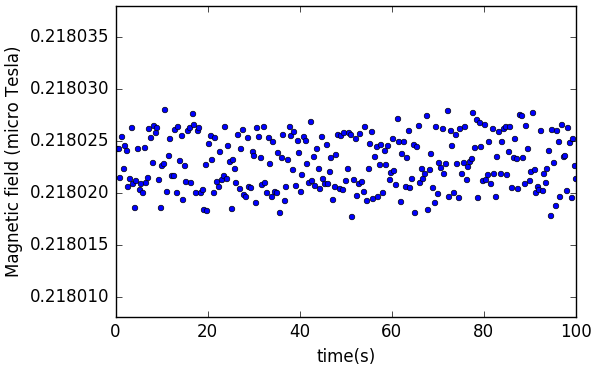
\includegraphics[width=\textwidth]{figures/beam_power_less}
        \caption{}
        \label{fig:power less}
    \end{subfigure}

    \begin{subfigure}[b]{0.7\textwidth}
        \centering
        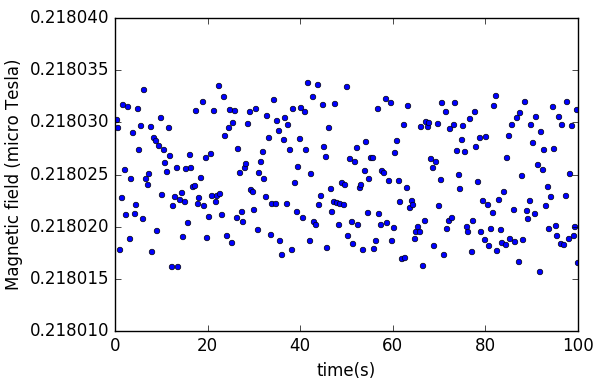
\includegraphics[width=\textwidth]{figures/beam_power_double}
        \caption{}
        \label{fig:power double}
    \end{subfigure}
    \caption{ Magnetic field as a function of time for different power of probe beam.(a) measured magnetic field with probe beam power 15 $\mu$w. Precession width is about $3.01$ pT (b) measured magnetic field with precession width $7.2$ pT for probe beam power 30 $\mu$w.}
    \label{fig:different probe power}
\end{figure}
%data colllected 13th August 2018
 
 In Fig \ref{fig:different probe power} the measured magnetic field has been displayed for two different  Probe beam power. Fig \ref{fig:power less} present the measured field over 100 s with 15 $\mu$W probe power while fig \ref{fig:power double} display the measured field over 100 s for probe power 30 $\mu$W. In both cases, the pump beam power has been kept unchanged ($\sim $40 $\mu$W). Each blue points in this graph represent a single FID scan. As can be seen from Fig \ref{fig:different probe power} the magnetic field is more scattered for high probe beam power. Precession width is about $7.2$ pT for probe beam power 30 $\mu$W while for low beam power(15 $\mu$W) the precession width is about $3.01$ pT. It can be concluded lower probe beam power is better for precession  magnetometry because the narrower the precession width more sensitive the magnetometer. Although low probe beam power is better for precise field measurement, it's hard to work with because of the dimness of light.
Table  \ref{table:Coherence time for different probe power} represent the coherence time for different probe power while the pump beam power was unchanged (120 $\mu$W).
 \begin{table}%[h]
\centering
\begin{tabular}{|l  |c|c|}\hline
\textbf{Probe power($\mu$w)}    & \textbf{Coherence time(ms)}  & \textbf{Amplitude(Volts)}\\\hline
~~~~~~~~2 & 84 & 2.13   \\
\hline
~~~~~~~~5    & 82 & 2.11  \\
\hline
~~~~~~~~10   &  68 & 4.06 \\
\hline
~~~~~~~~15  &   59 & 5.8  \\
\hline
~~~~~~~~35  &   32 & 10  \\
\hline
\end{tabular}
\caption{Coherence time for different probe power\label{table:Coherence time for different probe power}}
\end{table}
 
 \begin{figure}
    \centering  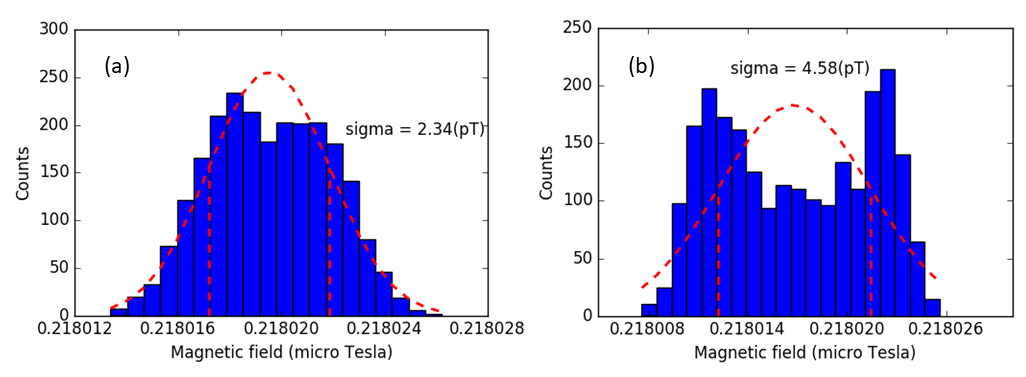
\includegraphics[width=\textwidth]{figures/pump_beam}
    \caption{ Magnetic field vs. time for different pump beam power. (a) measured magnetic field with duty cycle $5 \%$. Precession width is about $2.3$ pT (b) measured magnetic field with Precession width $4.6$ pT for  16 $\%$ duty cycle.}
    \label{fig:different pump power}
\end{figure}

Another study has been conducted to understand the influence of pump beam power on precession magnetometry. During this study, the probe beam power ($\sim$ 15 $ \mu$W) has kept unchanged while pump power has changed. In this measurement data has been acquired by running the magnetometer in FID mode. In FID mode amplitude modulation of pump beam has been done by using a AOM.  So the pump beam power can be change by changing the duty cycle of square wave modulation. When duty cycle is set to $5\%$ the pump beam power is 40 $\mu$W and for $16 \%$ duty cycle power is 128 $\mu$W. During this measurement the lock-in reference frequency was set to 1943.9 Hz while the AOM frequency was 2036 Hz. The histogram of measured magnetic field for different pump beam power has been showed in fig \ref{fig:different pump power}. The precession width (sigma) become larger for higher duty cycle while it becomes narrower for small duty cycle. In the case of 5$\%$  duty cycle precession width is about $2.3$ pT  (fig \ref{fig:different pump power}(a)) and for 16 $\%$ duty cycle the spread is about 4.6 pT (fig \ref{fig:different pump power}(b)). It is clear from the plot that, at higher duty cycle data points are not statistically distributed.  When a pump beam with a higher duty cycle is used  in precession magnetometry, the NMOR  signal amplitude increase accordingly. But it has been observed that error in frequency measurement also increases with higher signal amplitude which was not expected. A strong correlation between magnetic field and phase of the NMOR signal also has been observed for higher pump power. So it can be concluded that using higher duty cycle could induce more systematic errors in field measurement which led to the next study.


\subsection{How far the reference frequency of lock-in amplifier should set to measure field correctly}
  
  The measurement technique of FID signal has been discussed elaborately in sec \ref{sec:FID}. In order to capture the FID signal correctly, the reference frequency of lock-in amplifier is normally set to about 100 Hz apart from the resonance frequency. In this study we kept all other setting fixed only changed the Lock-in reference frequency and observed the effect of that on field measurement study. The measurement was conducted at $0.2 \mu$T field. 
   \begin{figure}
    \centering
    \begin{subfigure}[b]{0.4\textwidth}
        \centering
        \includegraphics[width=\textwidth]{figures/reference_frequency1}
        \caption{}
        \label{fig:far from resonance}
    \end{subfigure}
    \hfill
    \begin{subfigure}[b]{0.4\textwidth}
        \centering
        \includegraphics[width=\textwidth]{figures/reference_frequency3}
        \caption{}
        \label{fig: middle range}
    \end{subfigure}
    \begin{subfigure}[b]{0.4\textwidth}
        \centering
        \includegraphics[width=\textwidth]{figures/reference_frequency2}
        \caption{}
        \label{fig:close to resonance}
    \end{subfigure}
 \caption{FID signal for different reference frequency of Lock-in amplifier while the resonance frequency was 2035 kHz.(a) reference frequency was set to 92 Hz far from resonance (b) difference between resonance and reference frequency is 40 Hz, (c) reference frequency was set to 2015 Hz while resonance frequency 2035 Hz. \label{fig:different reference signal}}
\end{figure}

  \begin{figure}[h]
\centering\includegraphics[width=0.8\linewidth]{figures/freq_1943_single_fit_300microsec.png}
\caption{Lock-in reference frequency and time constant are 1943 Hz and 300$\mu$s respectively. The resonance frequency is 2035 Hz. In this case only x data was fitted. \label{fig:freq_1943_single_fit_300_micros}}
\end{figure}


  \begin{figure}[h]
\centering\includegraphics[width=0.8\linewidth]{figures/freq_1943_simultaneous_fit_300microsec_.png}
\caption{Lock-in reference frequency and time constant are 1943 Hz and 300$\mu$s respectively. In this case both x and y data was fitted simultaneously. \label{fig:freq_1943_simultaneous_fit_300_micro_sec}}
\end{figure}

 \begin{figure}[h]
\centering\includegraphics[width=0.8\linewidth]{figures/freq_2015_simultaneous_fit_300microsec.png}
\caption{Lock-in reference frequency and time constant are 2015 Hz and 300$\mu$s respectively. In this case both x and y data was fitted simultaneously. \label{fig:freq_2015_simultaneous_fit_300_micros}}
\end{figure}

  \begin{figure}[h]
\centering\includegraphics[width=0.8\linewidth]{figures/freq_1943_simultaneous_fit_1ms.png}
\caption{Lock-in reference frequency and time constant are 1943~Hz and 1~ms respectively.  \label{fig:freq_1943_simultaneous_fit_1ms}}
\end{figure}

  \begin{figure}[h]
\centering\includegraphics[width=0.8\linewidth]{figures/freq_2015_simultaneous_fit_1ms.png}
\caption{Lock-in reference frequency and time constant are set to 2015~Hz and 1~ms respectively. \label{fig:freq_2015_1ms}}
\end{figure}


 
  The FID signal for different reference frequency of lock-in amplifier has shown in Fig \ref{fig:different reference signal}. In the case of Fig \ref{fig:far from resonance} the reference frequency of lock-in was set to 1943.9 Hz (90 Hz far from resonance frequency). On the other hand for Fig \ref{fig:close to resonance} the reference frequency of lock-in was set to 2015 Hz (20 Hz far from resonance frequency). In this study the resonance frequency was always set to 2035 Hz and the pump power(~60 $\mu$w) and probe power (~32 $\mu$w)
  
  Fig\ref{fig:freq_1943_single_fit_300_micros} display the example of fitted FID signal(upper left figure), measured magnetic field over time (upper right figure), phase as a function of time (bottom left figure) and magnetic field vs. phase (bottom left figure) for lock-in reference frequency 1943 Hz. During this measurement the lock-in time constant was set to 300$\mu$~s. A clear indication of correlation between field and phase can be seen here.
  
   Fig\ref{fig:freq_1943_simultaneous_fit_300_micro_sec} display the example of simultaneous fitted x and y signal(upper left figure), measured magnetic field over time (upper right figure), magnetic field vs. phase (bottom left figure) and histogram of measured field (bottom left figure) for lock-in reference frequency 1943 Hz. During this measurement the lock-in time constant was set to 300$\mu$~s. 
   
    Fig\ref{fig:freq_2015_simultaneous_fit_300_micros} display the example of simultaneous fitted x and y signal(upper left figure), measured magnetic field over time (upper right figure), magnetic field vs. phase (bottom left figure) and histogram of measured field (bottom left figure) for lock-in reference frequency 2015 Hz. During this measurement the lock-in time constant was set to 300$\mu$~s.
    
    Fig \ref{fig:freq_1943_simultaneous_fit_1ms} display the example of simultaneous fitted x and y signal(upper left figure), measured magnetic field over time (upper right figure), magnetic field vs. phase (bottom left figure) and histogram of measured field (bottom left figure) for lock-in reference frequency 1943 Hz. During this measurement the lock-in time constant was set to 1~ms. 
    
  Fig \ref{fig:freq_2015_1ms} display the example of simultaneous fitted x and y signal(upper right figure), measured magnetic field over time (upper right figure), magnetic field vs. phase (bottom left figure) and histogram of measured field (bottom left figure) for lock-in reference frequency 1943 Hz. During this measurement the lock-in time constant was set to 1~ms.  
  
  In Fig \ref{fig:field for different lockin ref freq} the measured magnetic field over 35 s for different lock-in reference frequency has shown. It is obvious from the plot that if we set reference frequency very close to resonance frequency magnetic field start to oscillate. The exact reason behind this observed field oscillation remains unknown. We are thinking that when lock-in reference frequency is set very close to resonance frequency the fit function might fail to fit data properly due to the less zero crossings. So it seems like a systematic effect on field measurement rather than a real fact.
   
\begin{figure}[h]
\centering\includegraphics[width=0.8\linewidth]{figures/reference_frequency}
\caption{Measured magnetic field for different lock-in reference frequency. The red curve represents measured magnetic field when reference frequency was set to 2015 Hz which is 20 Hz far from resonance frequency. The blue curve shows magnetic field for lock-in reference frequency 1943.9 Hz. In this measurement only x data was fitted. \label{fig:field for different lockin ref freq}}
\end{figure}
   

\begin{figure}[h]
\centering\includegraphics[width=0.8\linewidth]{figures/sigma_diff_lock-in_frequency.png}
\caption{Histogram of the measured magnetic field for different lock-in reference frequency.\label{histogram-of-diff-lock-in freq}}
\end{figure}

  Table \ref{tab:FID_setting} represents all settings for FID NMOR. In this study the systematic effect of changing lock-in amplifier time constant on magnetic field measurement has been discussed.
  % \begin{figure}
   % \centering
   % \begin{subfigure}[b]{0.45\textwidth}
      %  \centering
       % \includegraphics[width=\textwidth]{figures/time_constant}
       % \caption{}
       % \label{fig:time constant long}
    %\end{subfigure}
    %\hfill
    %\begin{subfigure}[b]{0.45\textwidth}
       % \centering
       % \includegraphics[width=\textwidth]{figures/time_constant_300micro_sec}
       % \caption{}
        %\label{fig:time constant short}
    %\end{subfigure}
   % \caption{Histogram of measured magnetic field for different time constant of lock-in amplifier. (a) lock-in time constant was set to 1 ms (b) for lock-in time constant 300 $\mu$s. %\label{fig:different time constant} }
%\end{figure}
  
  %Fig \ref{fig:different time constant}  shows the histogram of measured magnetic field for two different time constant of lock-in amplifier while all other settings is same. In the case of Fig \ref{fig:time constant long} the lock-in time constant is 1 ms and Fig \ref{fig:time constant short} shows the histogram of magnetic field for time constant 300 $\mu$s. Here sigma is representing the precession width of field. It can be seen from the figure that the calculated sigma is larger for time constant 1 ms compared to 300 $\mu$s.  This measurements was conducted at 0.2 $\mu$T field. The resonance frequency and lock-in reference frequency are 2035 Hz and 1943 Hz respectively. The same study has also been done for higher lock-in reference frequency while resonance frequency was unchanged (2035 Hz). Fig: \ref{fig:diff time constant_high_frequency} display the histogram of the recorded magnetic field for different settings of time constant.
  
  
   %\begin{figure}
    %\centering
    %\begin{subfigure}[b]{0.45\textwidth}
        \centering
       % \includegraphics[width=\textwidth]{figures/2015_1ms.png}
       % \caption{}
        %\label{fig:time constant 1ms}
    %\end{subfigure}
    %\begin{subfigure}[b]{0.4\textwidth}
        %\centering
       % \includegraphics[width=\textwidth]{figures/2015_300micro_sec.png}
      %  \caption{}
       % \label{fig:time constant 300microsec}
    %\end{subfigure}
   % \caption{Histogram of measured magnetic field for different time constant of lock-in amplifier while lock-in frequency is set to 2015 Hz (20 Hz far from resonance frequency). (a) lock-in time constant was set to 1 ms (b) for lock-in time constant 300 $\mu$s. % for this measurement both x and y data were fitted simultaneously.
  %  \label{fig:diff time constant_high_frequency} }
%\end{figure}


%The magnetometric method based on FID NMOR is a very sensitive
%technique of magnetic field measurements. Those measurements are
%scalar, i.e., the position of a given resonance depends only on the
%magnitude not the direction of the magnetic field. However, the
%relative magnitudes of the FID NMOR resonances could have some
%dependency on the magnetic field direction. Thus there is a
%possibility to get some information about the direction of the
%magnetic field by doing a detailed analysis of the FID NMOR signal.
%For this reason, the dependency of the FID NMOR signal on the
%magnetic field direction has studied here.
\section{Study magnetometer performance with tilted field} 
\label{sec:tilted-results}

 %\begin{figure}
    %\centering
    %\begin{subfigure}[b]{0.45\textwidth}
       % \centering
       % %\includegraphics[widt%h=\textwidth,trim={0cm 0.5cm 0cm 0cm},clip]{figures/tilt1.png}
        %\caption{}
        %\label{fig:tilt_0_degree}
    %\end{subfigure}
   % \caption{Optical rotation as a function of time at $\Omega_L$ in the yz plane for different tilt angle.\label{fig:optical-rotation-different-angle}}
%\end{figure}

\begin{figure}
  \centering
%trim={<left> <lower> <right> <upper>}
\includegraphics[width=0.8\textwidth]{figures/tilted_field_scope_trace.png}
  \caption{Optical rotation as a function of time at $\Omega_L$ in the yz plane for different tilt angle. When tilt angle is 0$\degree$ the FID signal contain only one frequency component but the signal contain two frequency component for tilt angle 15$\degree$ and 40$\degree$.  \label{fig:optical-rotation-different-angle}}
    \label{fig:tilted}
\end{figure}
In this Rb NMOR magnetometry setup the rubidium atoms interacted with a $z$-directed laser light beam which is linearly polarized
along the y axis. In the FID NMOR technique, the magnetic field is generally directed along the light propagation direction and the resonance occurs at $2\Omega_L$.  This effect can be explained by considering that the polarization returns to its original state after a $180\degree$ rotation because of the two-fold symmetry of the optically pumped state. As a result, the optical rotation induced by the rotating linear dichroism is periodic at twice the Larmor frequency.

We have observed that Resonances in nonlinear magneto-optical rotation with amplitude modulated light by tilting the magnetic field at angles away from the direction of light propagation while operating the Rb magnetometer in FID mode. When the field is tilted in the plane perpendicular to the light polarization direction an resonance appears at $2\Omega_L$. In this case no additional resonance appears for modulation frequency $\Omega_L$. The amplitude of the FID NMOR signal decreases with increasing tilt angle. 

However, We also observed that by tilting the field direction toward the light polarization direction a new resonance occurs at $\Omega_L$ along with the main resonance at $2\Omega_L$. The resonance signal recorded at $\Omega_L$ contains two frequency components.
\begin{figure}[h]
\centering\includegraphics[width=0.7\linewidth]{figures/fft_amp.png}
\caption{FFT of FID  signal in the presence of transverse field at modulation frequency $\Omega_L$ while tilted the magnetic field direction toward light polarization direction  .\label{fig:fft-amplitude}}
\end{figure}


When direction of the magnetic is tilted toward the light polarization axis  the FID signal contain two frequency component at modulation frequency $\Omega_L$. Fig: \ref{fig:optical-rotation-different-angle} shows the FID signal for different tilt angle when pump beam is modulated at $\Omega_L$. In order to extract frequency components we have used two methods. One of them is the FFT of FID signal and the other one is the fit FID signal using equation \ref{eq:two_sinewave}.

\begin{equation}
     X = A_1 e^{-t /\tau_1} \sin(\omega_1 t + \phi_1) + A_2 e^{-t /\tau_2}  \sin (\omega_2 t + \phi_2) + C  
     \label{eq:two_sinewave}
\end{equation}

Where $A_1$ and $A_2$ are amplitude for two decaying sin wave, $\omega_1$ and $\omega_2$ represents oscillation frequency, $\phi_1$ and $\phi_2$ indicate phase and $\tau_1$ and $\tau_2$ represents coherence time. A 10th order Infinite Impulse Response( IIR) Butterworth filter is also used to reduce background noise from the signal.
Fig: \ref{fig:fft-amplitude} display the FFT of resonance signal for three different  tilt angle $0\degree$, $25\degree$ and $50\degree$. It can be seen from the plot that at $0\degree$ tilt angle there is only one frequency component while for $25\degree$ tilt angle two peak corresponds to two frequency components.

Fig.~\ref{fig:tilted-wrong} shows the amplitude of the FID signal for the magnetic field tilted in the $xz$ plane at various angles to the light propagation direction at modulation frequency $2\Omega_L$ and $\Omega_L$. It can be seen from the figure that the amplitude of the FID signal decreases with increasing tilt angle for both modulation frequency. 

\begin{figure}
    \centering
   \begin{subfigure}[b]{0.45\textwidth}
        \centering
        \includegraphics[width=\textwidth]{figures/tilt_x_larmor.png}
        \caption{}
        \label{fig:y equals x}
    \end{subfigure}
    \hfill
     \begin{subfigure}[b]{0.45\textwidth}
        \centering
        \includegraphics[width=\textwidth]{figures/tilt_x_2larmor.png}
        \caption{}
        \label{fig:three sin x}
    \end{subfigure}
    \caption{ The amplitude of the FID NMOR signals as a function
      of tilt angle recorded at $\Omega_L$ and $2\Omega_L$ vs. the
      tilt angle of the magnetic field in the plane defined by the
      light-polarization and light propagation vectors (xz-plane). \label{fig:tilted-wrong}}
\end{figure}

\begin{figure}
    \centering
   \begin{subfigure}[b]{0.45\textwidth}
        \centering
        \includegraphics[width=\textwidth]{figures/tilt_y_larmor.png}
        \caption{}
        \label{fig:tilt_y}
    \end{subfigure}
    \hfill
     \begin{subfigure}[b]{0.45\textwidth}
        \centering
        \includegraphics[width=\textwidth]{figures/tilt_y_2larmor.png}
        \caption{}
        \label{fig:tilt_x}
    \end{subfigure}
    \caption{(a) The amplitude of the FID NMOR signals as a function
      of tilt angle recorded at $\Omega_L$ and $2\Omega_L$ vs. the
      tilt angle of the magnetic field in the plane defined by the
      light-polarization and light propagation vectors(yz-plane). \label{fig:something-tilted}}
\end{figure}

Fig.~\ref{fig:something-tilted}(a) indicates the signal amplitude vs. different tilt angle at $\Omega_m=2\Omega_L$ . The amplitude of resonance signal at $2\Omega_L$  decreases as the angle between magnetic field $B$ and the light propagation direction increases while the amplitude of new resonance  increases with increasing tilt angle at $\Omega_L$.
      
Fig.~\ref{fig:something-tilted}(b) shows the resonance amplitude at $\Omega_m=2\Omega_L$ keep decreases with increasing tilt angle in $yz$ plane while  the resonance amplitude measured at $\Omega_m=\Omega_L$ keep increase till $30\degree$ and after that amplitude start to decrease and reaches zero when the magnetic field is directed along the y axis. For both cases (Fig: \ref{fig:tilted-wrong} and Fig:\ref{fig:something-tilted}) the signal amplitude has been extracted as a fit parameter when data was fitted to the fit function \ref{eq:two_sinewave}
\begin{figure}[h]
\centering\includegraphics[width=0.9\linewidth]{figures/fitted_data_tilted_field.png}
\caption{(a) Fitted FID signal using Eq. \ref{eq:two_sinewave}. (b)  The zoomed version of (a). The  blue line indicates raw data while the red one indicates fitted curve}
\end{figure}
\begin{figure}[h]
\centering\includegraphics[width=0.9\linewidth]{figures/filtered_data.png}
\caption{(a)Raw and filtered FID signal. (b) zoomed version of (a)}
\end{figure}

Consider a two-level system $F=1\rightarrow F=0$ and the quantization vector is directed along the magnetic field. When the magnetic field is tilted in the yz plane, the light-polarization axis is perpendicular to the magnetic field. In this case the linearly polarized light containing two circularly polarized components can only create the coherence state between magnetic sublevels $m_F=\pm 1$ . Since the transition frequency between these two consecutive Zeeman energy sublevels is $2\Omega_L$  the resonance appears only at this frequency. 

However, when the magnetic field is tilted  in the xy plane, the light is a linear superposition of polarizations parallel and perpendicular to the magnetic field. In this case, the light can create coherences between sublevels with $m_F=1$ and $m_F=2$, so resonances are observed at both $ \Omega_L$ and 2$\Omega_L$. 
 

\chapter{}
\section{Conclusion}
\section{Future work}
\begin{itemize}
\item	FEMM simulation of z-coil 	Homogeneity of z-coil in this shielding configuration is not known or measured.  (Never measured with endcaps of innermost shield removed.)
\begin{itemize}
\item Probably this is to compare with Junyao’s coil and its homogeneity

\item
Can also measure homogeneity of z-coil in shield – it has been done before and I recall that it is homogeneous at $\% $level when in shield with basic degaussing (not our present degaussing system).
\end{itemize}
\item
Study magnetometer performance with Junyao's coil inside shield. 
\begin{itemize}
\item	The idea here is to show whether decoupling the coil from the shield has any impact on long-term stability.
 \item removing the lock-in amplifier
\end{itemize}
\end{itemize}
\newpage
\printbibliography
\end{document}


